% Some kind of 35t analysis -- looking at pi0s in 35t
% Target: 30 pages

\graphicspath{{35tonAnalysis/Figs/}}

%%%%%%%%%%%%%%%%%%%%%%%%%%%%%%%%%%%%%%%%%%%%%%%%%%%%%%%%%%%%%%%%%%%%%%%%%%%%%%%%%%%%%%%
\chapter{Analysis of 35~ton Data}\label{chap:35tAnalysis}

The 35~ton run (see Section \ref{chap:35ton}) provided 22 days of good quality (high purity, stable field ($250$~V/cm), stable DAQ), analysable data.  Due to the issues encountered, high quality physics analyses proved very challenging and instead more time was taken developing software to mitigate issues such as coherent noise and digitiser stuck bits.  Analyses, particularly those presented here, focused on trying to understand the detector and characterise previously untested responses.  In this respect, the 35~ton proves to be a vital experiment in informing the next generation of prototypes and even the final DUNE far detector design.  It also boasts datasets which no planned experiment will before the full DUNE modules; it is therefore essential as much information as possible is extracted from the 35~ton analyses.

Before analyses are presented, techniques developed to enhance the quality of the data, and the data selection, will be discussed in Section \ref{sec:Preparing35tonData}.  A short section demonstrating how LAr purity may be determined from data is contained in Section \ref{sec:PurityAnalysis} before the main analyses, concerning tracks passing through the APA frames and across APA gaps, are presented in Section \ref{sec:APACrossing} and Section \ref{sec:APAGapCrossing} respectively.  Finally, a brief investigation into the performance of basic shower and calorimetric reconstruction on the 35~ton data is discussed in Section \ref{sec:ShowerData}.

%%%%%%%%%%%%%%%%%%%%%%%%%%%%%%%%%%%%%%%%%%%%%%%%%%%%%%%%%%%%%%%%%%%%%%%%%%%%%%%%%%%%%%%
\section{Preparing 35~ton Data for Analysis}\label{sec:Preparing35tonData}

To ensure analyses are as accurate as possible, careful pre-selection and preprocessing of the data is performed.  Methods for producing the analysable sample are discussed in the section.

%%%%%%%%%%%%%%%%%%%%%%%%%%%%%%%%%%%%%%%%%%%%%%%%%%%%%%%%%%%%%%%%%%%%%%%%%%%%%%%%%%%%%%%
\subsection{Selecting the Data}\label{sec:SelectingTheData}

The level of noise present in the TPC data varied hugely between runs -- this is evident from analysing the RMS of the charge read out on a particular channel.  Figure \ref{fig:DataRMS} shows a comparison of this metric for `good' and `bad' runs.

\begin{figure}[h]
  \centering
  \begin{subfigure}{0.45\linewidth}
    \centering
    \includegraphics[width=0.95\textwidth]{DataRMSGood.pdf}
    \caption{Good run}
    \label{fig:DataRMSGoodRun}
  \end{subfigure}
  \hfill
  \begin{subfigure}{0.45\linewidth}
    \centering
    \includegraphics[width=0.95\textwidth]{DataRMSBad.pdf}
    \caption{Bad run}
    \label{fig:DataRMSBadRun}
  \end{subfigure}
  \caption[`Good' and `bad' 35~ton runs]{Comparison between noise levels for `good' and `bad' 35~ton runs.  The channels shown are on APA2 (online convention, APA0 offline) and are read out by RCEs 8 through 11 (labelled).  The increase in read out charge RMS in evident in the case of the noisy run.  These plots are from runs 15797 (Fig \ref{fig:DataRMSGoodRun}) and 15790 (Figure \ref{fig:DataRMSBadRun}) and were taken only 50 minutes apart.}
  \label{fig:DataRMS}
\end{figure}

Runs which exhibited the lowest noise were selected for analysis.  In all there were 1269 runs used representing some data taken before the FNAL site wide power outage (3rd March 2016) with most the week after stabilising the experiment again (9th March -- 17th March).  A selection of bad channels, classified as either `dead' (electrically) or `bad' (exhibit sufficiently more than average noise), represent 8\% of the total number of channels.

Due to the continuous nature of data taking, there is a non-trivial correlation between a `DAQ event', a collection of fragments read out by the DAQ, and a `physics event', an event in which particle interactions occurred.  The external triggers used in the 35~ton, namely the external muon scintillators and the photon detectors, are used to define the event time.  Given the trigger rate at which most data was taken ($\sim1$~Hz), a typical run comprising a few thousand events will only contain $\mathcal{O}(10)$ triggered events.  Furthermore, given the data format, these events often straddle multiple DAQ events (refer to Figure \ref{fig:TriggeredEvent} for a demonstration of this).  A splitter/stitcher module is employed to search for triggers within runs and construct physics events containing the useful information for analysis.  This produces a file with just this relevant information, which are then used for analysis.

%%%%%%%%%%%%%%%%%%%%%%%%%%%%%%%%%%%%%%%%%%%%%%%%%%%%%%%%%%%%%%%%%%%%%%%%%%%%%%%%%%%%%%%
\subsection{Improving Data Quality}\label{sec:ImprovingDataQuality}

Two issues present in the raw data, namely the presence of correlated noise and the stuck bits in the digitiser, are dealt with as an initial step of the reconstruction.  First, an algorithm attempting to correct for the stuck bits analyses waveforms on a wire and identifies problematic ADCs; interpolating between charges read out at neighbouring times is successful at reconstructing the initial waveform in most cases.  Figure \ref{fig:StuckBitInterpolation} demonstrates this interpolation method on simulated data.

\begin{figure}[h]
  \centering
  \includegraphics[width=8cm]{stuckbitsremoval.png}
  \caption[Correcting for stuck codes in the 35~ton data]{Simulated demonstration of the method used to correct for stuck codes in the 35~ton data.  On a given channel, ADCs exhibiting the consequences of this problem are corrected by interpolating charge at neighbouring time units.  This is tested by simulating a waveform and adding the observed stuck code effect; the efficacy of the method at correcting the afflicted bits can then be evaluated.}
  \label{fig:StuckBitInterpolation}
\end{figure}

The effect of applying this algorithm on a full waveform, to correct for all the stuck bits, is apparent in Figure \ref{fig:StuckBitWaveform}.

\begin{figure}[ht]
  \centering
  \begin{subfigure}[t]{0.48\linewidth}
    \centering
    \includegraphics[width=\textwidth]{raw_stuck.eps}
    \caption{Raw waveform before correcting for stuck bits.}
    \label{fig:StuckBitWaveformStuck}
  \end{subfigure}
  \hfill
  \begin{subfigure}[t]{0.48\linewidth}
    \centering
    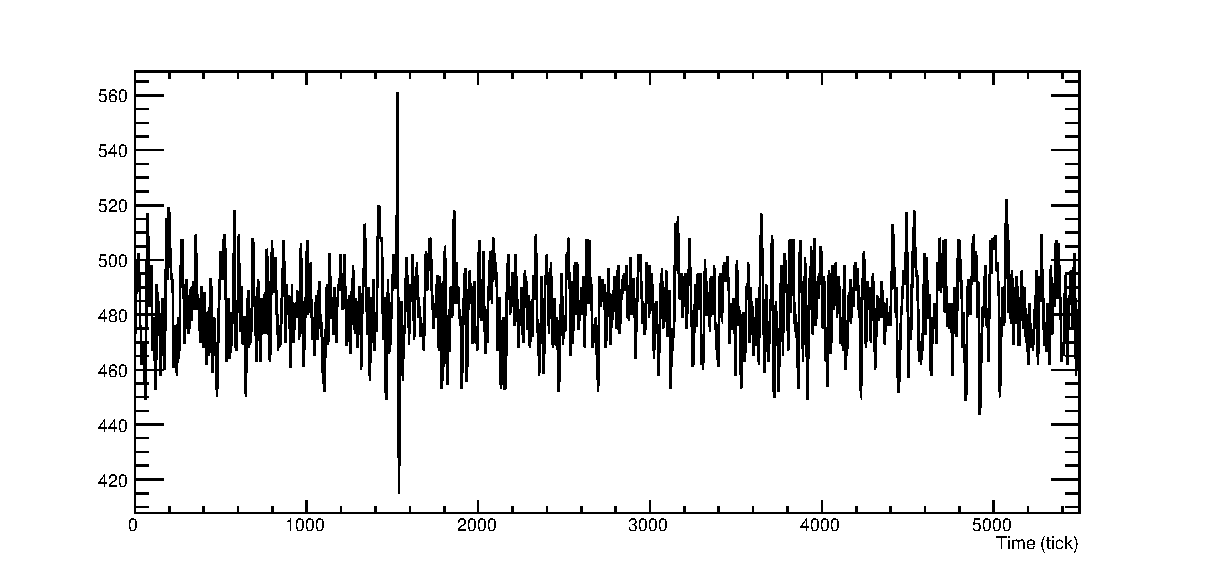
\includegraphics[width=\textwidth]{raw_unstuck.eps}
    \caption{After applying stuck bit mitigation.}
    \label{fig:StuckBitWaveformUnstuck}
  \end{subfigure}
  \caption[Raw data stuck bit mitigation]{The effect of applying stuck bit mitigation to a waveform as seen in raw data.  This particlular waveform is from run 15660, channel 722 (induction channel).}
  \label{fig:StuckBitWaveform}
\end{figure}

Following this process, a coherent noise removal stage is applied.  This simply looks at the average noise across channels sharing a front-end voltage regulator and removes this component from the readout ADC for each channel.  The effect of this correction is seen in Figure \ref{fig:CoherentNoiseRemoval}.

\begin{figure}[ht]
  \centering
  \begin{subfigure}[t]{0.48\linewidth}
    \centering
    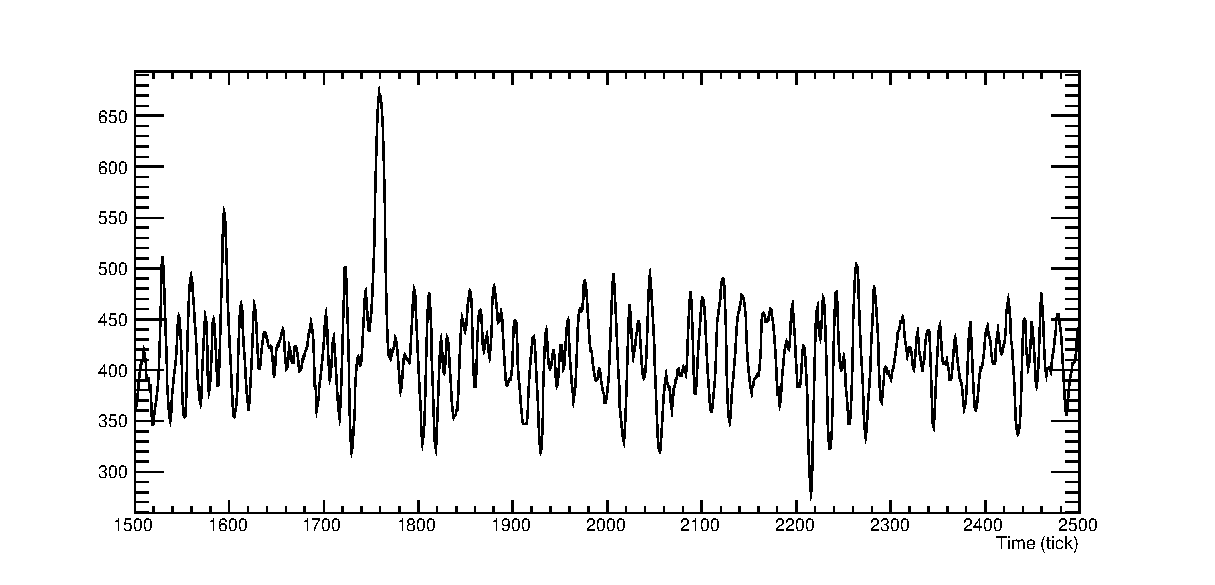
\includegraphics[width=\textwidth]{raw_noise.eps}
    \caption{Waveform before removing coherent noise.}
    \label{fig:CoherentNoiseRemovalNoise}
  \end{subfigure}
  \hfill
  \begin{subfigure}[t]{0.48\linewidth}
    \centering
    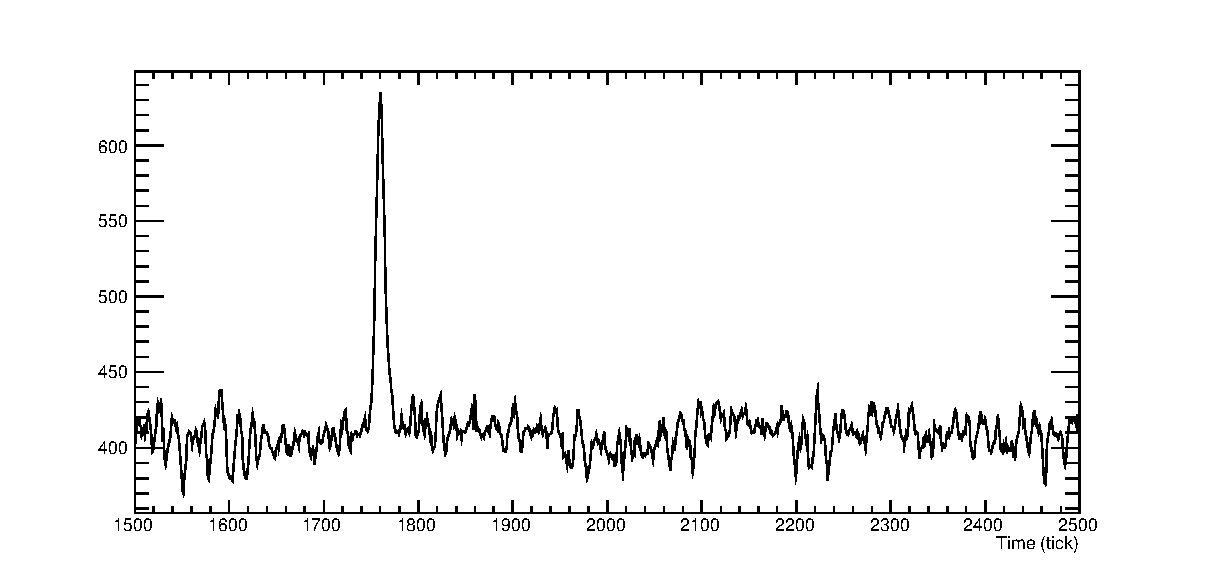
\includegraphics[width=\textwidth]{raw_nonoise.eps}
    \caption{After removing coherent noise.}
    \label{fig:CoherentNoiseRemovalNoNoise}
  \end{subfigure}
  \caption[Coherent noise removal in 35~ton data]{The effect of removing coherent noise from all channels on a voltage regulator.  This waveform is from run 15660, channel 2010 (collection channel).  The signal is noticably larger following this process, considerably improving reconstruction performance.}
  \label{fig:CoherentNoiseRemoval}
\end{figure}

%%%%%%%%%%%%%%%%%%%%%%%%%%%%%%%%%%%%%%%%%%%%%%%%%%%%%%%%%%%%%%%%%%%%%%%%%%%%%%%%%%%%%%%
\subsection{Reconstructing Muon Tracks}\label{sec:ReconstructingMuonTracks}

All analyses discussed below only make use of information recorded on the collection planes.  Since the induction wires are longer (a necessity for wrapping), a larger capacitance results in higher noise levels, complicating the reconstruction.  In general, after applying the refinements outlined in Section \ref{sec:ImprovingDataQuality}, the signals on the collection channels are prominent enough for competant analyses.  The methods used to select tracks are described in this section and applied during the subsequent studies.

Using only the collection plane presents challenges, the most obvious being the impossibility of full 3D reconstruction.  A hit on a collection wire at a given time gives well-defined $x$ and $z$ coordinates but cannot give any information in the $y$-direction.  `Quasi-3D' reconstruction is achieved by making use of the external counters.  Through-going muons are triggered by the coincidence of hits in two opposite counters; this information can be used to give a crude handle on the $y$ position of hits.

Figure \ref{fig:TrackSelection} outlines the stages of selecting hits originating from the particle track which caused the trigger.  Figure \ref{fig:TrackSelectionBefore} shows all hits from an example event containing a through-going muon.  The first stage of track selection involves taking those hits which lie in the `counter shadow', the narrow section of collection plane area physically inbetween the opposing counters through which the triggering particle passed.  The hits which remain are shown in Figure \ref{fig:TrackSelectionCounterShadow}.  The track hits are visible along with further, unrelated hits.  These are removed by requiring that only hits on wires with single occupancy be kept, and then applying a linear fit and removing all hits with residual $>2$~cm.  The final output after these stages is shown in Figure \ref{fig:TrackSelectionFinal}.

\begin{figure}[ht]
  \centering
  \begin{subfigure}[t]{0.48\linewidth}
    \centering
    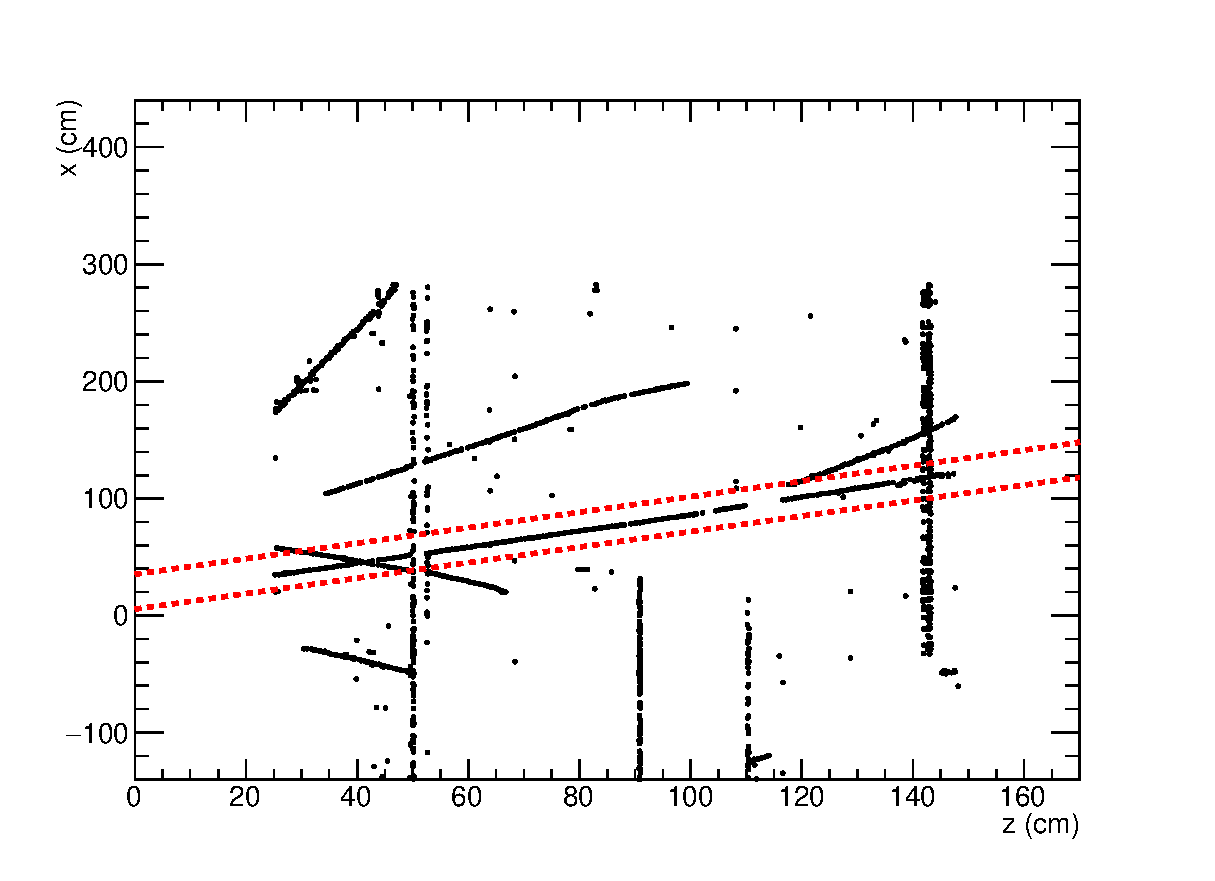
\includegraphics[width=\textwidth]{hitselection_all.eps}
    \caption{All hits before any track selection.  The red lines represent the boundary defined by the edges of the two counters causing the trigger.}
    \label{fig:TrackSelectionBefore}
  \end{subfigure}
  \hfill
  \begin{subfigure}[t]{0.48\linewidth}
    \centering
    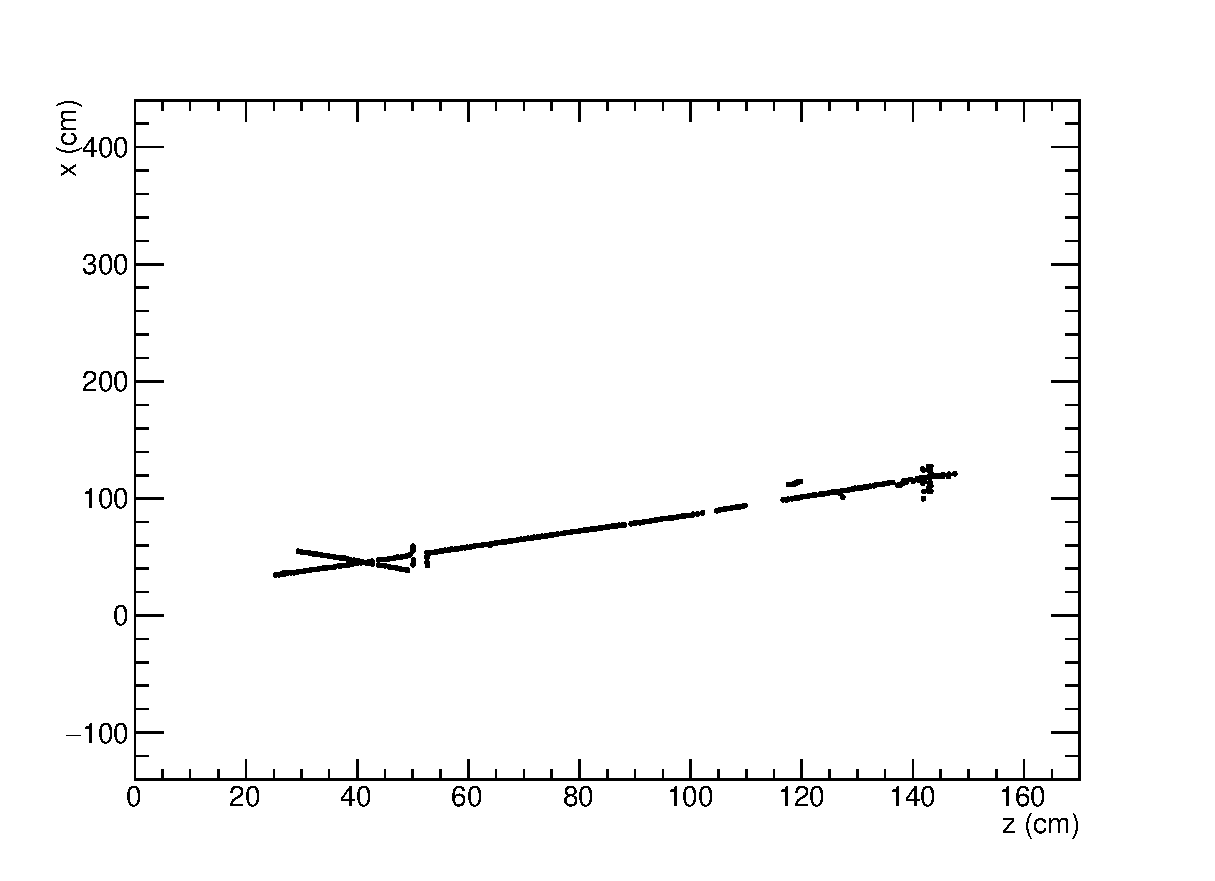
\includegraphics[width=\textwidth]{hitselection_shadow.eps}
    \caption{Hits in the counter shadow.}
    \label{fig:TrackSelectionCounterShadow}
  \end{subfigure}
  \hfill
  \begin{subfigure}[t]{0.48\linewidth}
    \centering
    \includegraphics[width=\textwidth]{hitselection_final.eps}
    \caption{Hits on single wire occupancy and with residual $<2$~cm.}
    \label{fig:TrackSelectionFinal}
  \end{subfigure}
  \caption[Selecting tracks for 35~ton data analysis]{Demonstration of the successive stages applied to hits on collection wires in order to select hits from the through-going track associated with the particle which caused the trigger.  The hits left after all stages are taken forward into the analyses.}
  \label{fig:TrackSelection}
\end{figure}

The result of this track selection, as evident from Figure \ref{fig:TrackSelectionFinal}, is a well-formed, high quality track with which it is possible to perform analyses.  These will be the focus of the remainder of this chapter.

%%%%%%%%%%%%%%%%%%%%%%%%%%%%%%%%%%%%%%%%%%%%%%%%%%%%%%%%%%%%%%%%%%%%%%%%%%%%%%%%%%%%%%%
\section{Measuring LAr Purity from Crossing Muons}\label{sec:PurityAnalysis}

%%%%%%%%%%%%%%%%%%%%%%%%%%%%%%%%%%%%%%%%%%%%%%%%%%%%%%%%%%%%%%%%%%%%%%%%%%%%%%%%%%%%%%%
\section{APA-Crossing Muons}\label{sec:APACrossing}

The 35~ton is the only proposed experiment before the full DUNE far detector modules that have fully implemented anode planes within the cryostat reading out data from multiple drift regions simultaneously (ProtoDUNE will have wrapped wire APAs but will only read out one drift region each and SBND has the CPAs in the centre of the cryostat with the APAs at the edges).  Referring to Figure \ref{fig:DUNEFarDetectorDesign}, this is a design consideration that features prominantly in the eventual detector so any implications in the data must be well understood.  Analysis of tracks which pass through the APAs and deposit charge in both drift regions is the subject of this section.

In Section \ref{sec:APACrossingT0}, a method to determine the absolute event time, T0, from APA crossing tracks is presented and in Section \ref{sec:APACrossingCharge} the charge deposited by these tracks, particularly when crossing through the planes, is studied.  Comparisons between the two drift regions, made possible by comparing tracks left by the same particle, are contained in Section \ref{sec:APACrossingDriftComparison}.

%%%%%%%%%%%%%%%%%%%%%%%%%%%%%%%%%%%%%%%%%%%%%%%%%%%%%%%%%%%%%%%%%%%%%%%%%%%%%%%%%%%%%%%
\subsection{T0 Determination from APA Crossing Tracks}\label{sec:APACrossingT0}

Given the nature of a TPC detector, an `event time' (T0) must be known in order to set an absolute timescale, and therefore absolute position, on all interactions within the detector.  An accurate T0 is essential for calorimetric reconstruction: in order to understand how much charge a hit had when it was created, a lifetime correction dependent on the total drift time must be applied.  An incorrect T0 would lead to a systematic under- or over-estimation of the reconstructed energy and have implications in particle identification and shower energy determination.

In a LArTPC, an event time is usually given by an external triggering system.  The DUNE far detector will rely on the instantaneous detection of photons produced from the immediate recombination of the ionisation electrons with positive Ar ions.  In the 35~ton, an additional external system was provided by the scintillation counters.  Since the sample of APA crossing muons used in this analysis were all selected and reconstructed using counter information, an interaction time is immediately known.

Without correctly accounting for T0, the tracks on each side of the APAs appear offset from the planes.  This is evident from the event display shown in Figure \ref{fig:evd_t0}.  By aligning the track segments on either side of the APAs, a measurement of T0 can be made directly from the TPC data.

\begin{figure}[ht]
  \centering
  \includegraphics[width=10cm]{evd_t0_2.pdf}
  \caption[Event display showing the effect of unaccounting for T0]{Event display made during the run in which a track passes through the APAs.  Correcting for T0 would eliminate the visible offset and result in a single accurately connected track.}
  \label{fig:evd_t0}
\end{figure}

%%%%%%%%%%%%%%%%%%%%%%%%%%%%%%%%%%%%%%%%%%%%%%%%%%%%%%%%%%%%%%%%%%%%%%%%%%%%%%%%%%%%%%%
\subsubsection{Aligning APA Crossing Tracks}\label{sec:APACrossingAlignment}

Two complementary methods were used to accurately align the track segments across the APA.  Both involved initially correcting for the counter T0, $T_0^{\mathrm{counter}}$, before considering a range of alternative T0 hypotheses and minimising a relevant metric to determine the most likely value.  In the first method, demonstrated in Figure \ref{fig:APACrossingAlignmentLeastSq}, a least square linear fit is applied to the track and the residual minimised.  The second method, demonstrated in Figure \ref{fig:APACrossingAlignmentSeparation}, involves fitting a line to each segment in turn and minimising the projected distance between the intersections of the lines with the centre of the APAs ($x=0$).  As will shown later, and can be seen from Figs. \ref{fig:APACrossingAlignmentLeastSqMin} and \ref{fig:APACrossingAlignmentSeparationMin}, the two methods agree very well with each other.

\begin{figure}[p]

  \centering

  \begin{subfigure}[t]{0.48\linewidth}
    \centering
    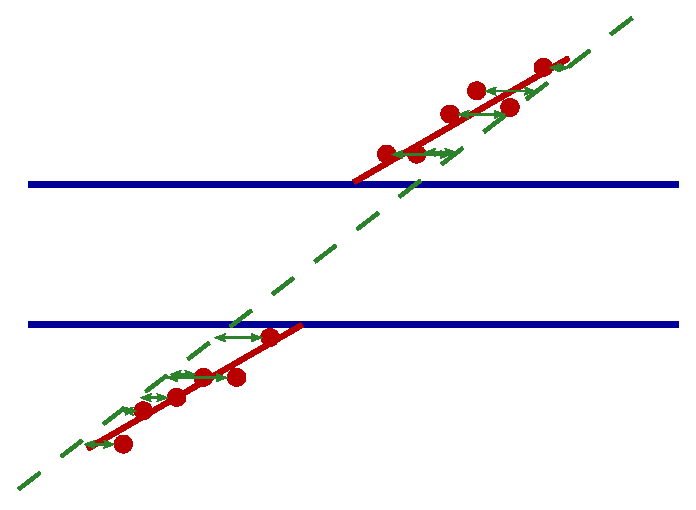
\includegraphics[width=\textwidth]{track_residual.eps}
    \caption{Demonstration of the calculation of residuals from a linear fit through all hits.  The red points are hits and the green line represents a linear fit through all points on both sides of the APA.}
    \label{fig:APACrossingAligmentLeastSqResidual}
  \end{subfigure}
  \hfill
  \begin{subfigure}[t]{0.48\linewidth}
    \centering
    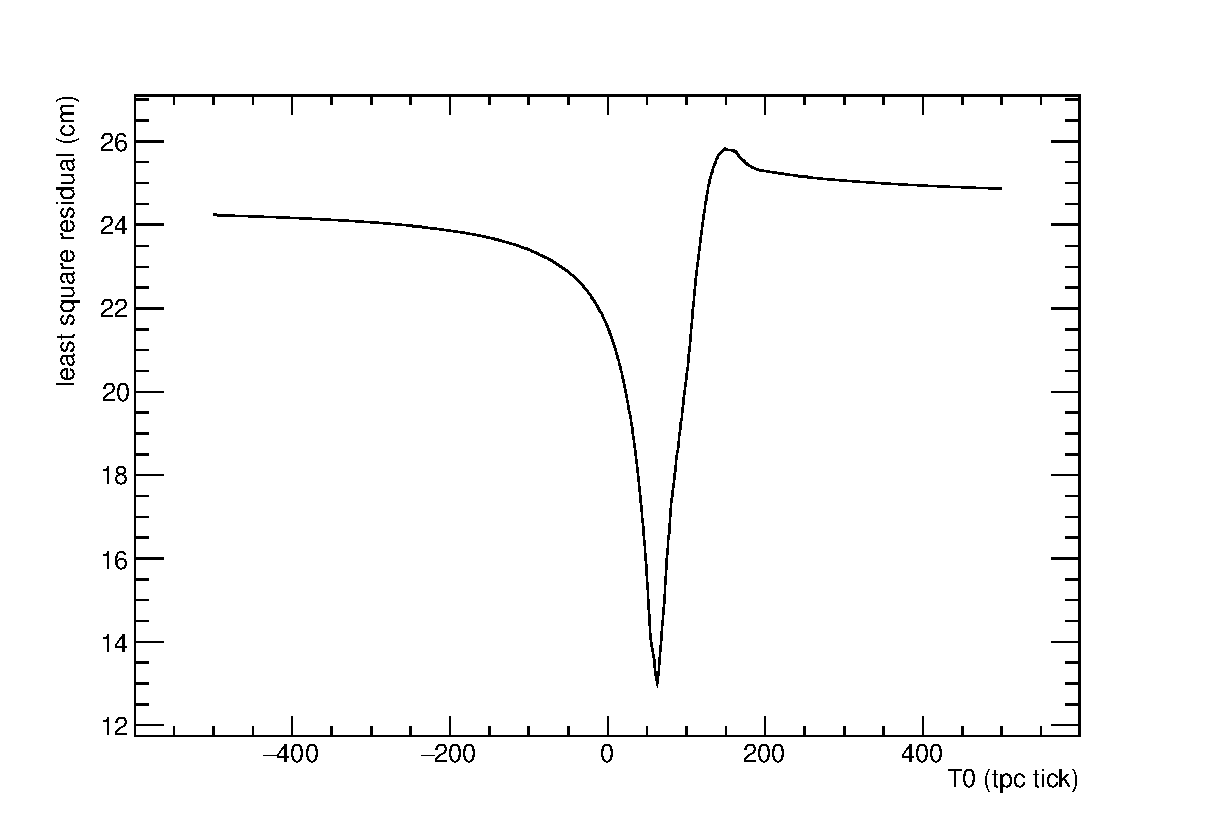
\includegraphics[width=\textwidth]{chisquare.eps}
    \caption{The residuals to the linear fit of the track over a range of T0 candidates.  The value of T0 which minimises this distribution (62 ticks in this case) is considered the most likely intereaction time.}
    \label{fig:APACrossingAlignmentLeastSqMin}
  \end{subfigure}
  \caption[Method to align track segments on either side of the APAs involving minimising residuals from linear least square fit.]{Method to align track segments on either side of the APAs involving minimising residuals from a linear least square fit.  A fit is applied to all hits and the resulting residual, a representation of the `goodness of fit', is minimised over a range of T0 candidates to find the most likely interaction time for the particle leaving the track.}
  \label{fig:APACrossingAlignmentLeastSq}

  \vspace*{\floatsep}

  \begin{subfigure}[t]{0.48\linewidth}
    \centering
    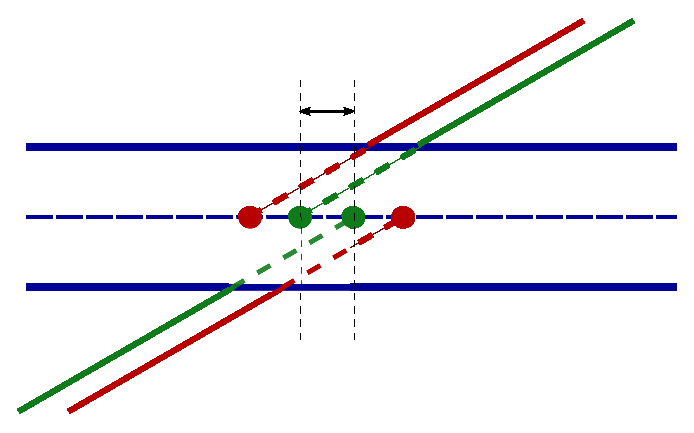
\includegraphics[width=\textwidth]{track_separation.eps}
    \caption{Demonstration of the determination of the distance between the track segments at the centre of the APAs.  The red and green lines represent linear fits to the hits (applied separately on each side of the APA) for different values of T0.}
    \label{fig:APACrossingAligmentLeastSqSeparation}
  \end{subfigure}
  \hfill
  \begin{subfigure}[t]{0.48\linewidth}
    \centering
    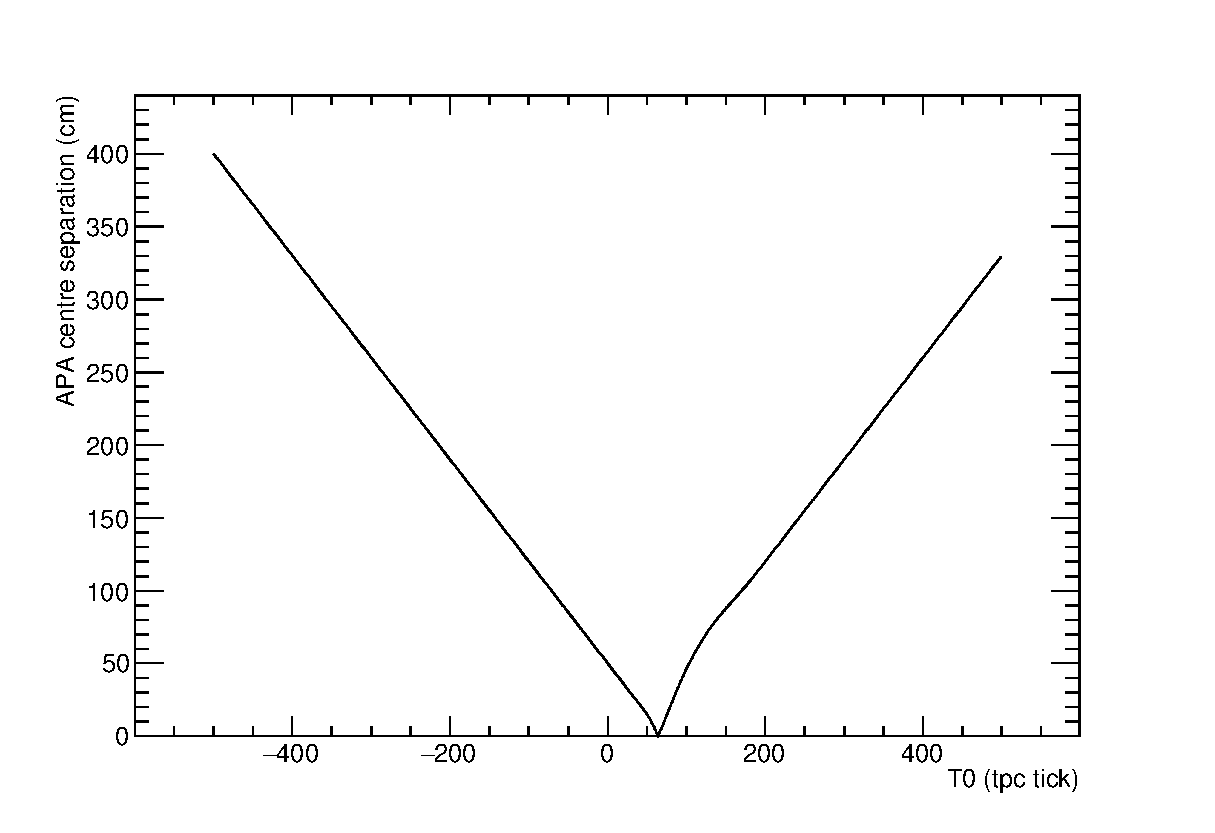
\includegraphics[width=\textwidth]{separation.eps}
    \caption{The separation distance over a range of T0 candidates.  The value of T0 which minimises this distribution (63 ticks in this case) is considered the most likely interaction time.}
    \label{fig:APACrossingAlignmentSeparationMin}
  \end{subfigure}
  \caption[Method to align track segments on either side of the APAs involving minimising the distance between the projected intersection of each with the centre of the APAs.]{Method to align track segments on either side of the APAs involving minimising the distance between the projected intersection of each with the centre of the APAs.  A fit is applied to each track segment separately and the distance between the intersection of these lines with the centre of the APA in minimised over a range of T0 candidates to find the most likely interaction time for the particle leaving the track.}
  \label{fig:APACrossingAlignmentSeparation}

\end{figure}

Naively, one would expect the T0 determined using these methods, $T_0^{\mathrm{TPC}}$, to agree with $T_0^{\mathrm{counter}}$.  It was noted however that there appeared to be a systematic offset between the T0 given by the counters and measured from the TPC data.  The distribution of this disparity is shown in Figure \ref{fig:TPCCounterT0Difference}; it peaks very sharply around 64 ticks (32~$\mu$s) and is importantly inconsistent with zero.  This suggests an inconsistency somewhere in the data taking and will be the subject of the remainder of this section.  Figure \ref{fig:TPCCounterT0Correction} shows an example track before and after this disparity is corrected for.

\begin{figure}
  \centering
  \includegraphics[width=14cm]{TPCCounterT0Difference.eps}
  \caption[Difference between the T0 calculated from TPC data and the T0 provided by the counters representing the trigger time of the through-going muon.]{[Placeholder image until I get one with full stats again!] Difference between the T0 calculated from TPC data and the T0 provided by the counters representing the trigger time of the through-going muon.  If the two measurements of T0 agreed the distribution would peak at zero; the fact it does not is indicative of a systematic offset somewhere in the data taking.}
  \label{fig:TPCCounterT0Difference}
\end{figure}

\begin{figure}
  \centering
  \begin{subfigure}[t]{0.48\linewidth}
    \centering
    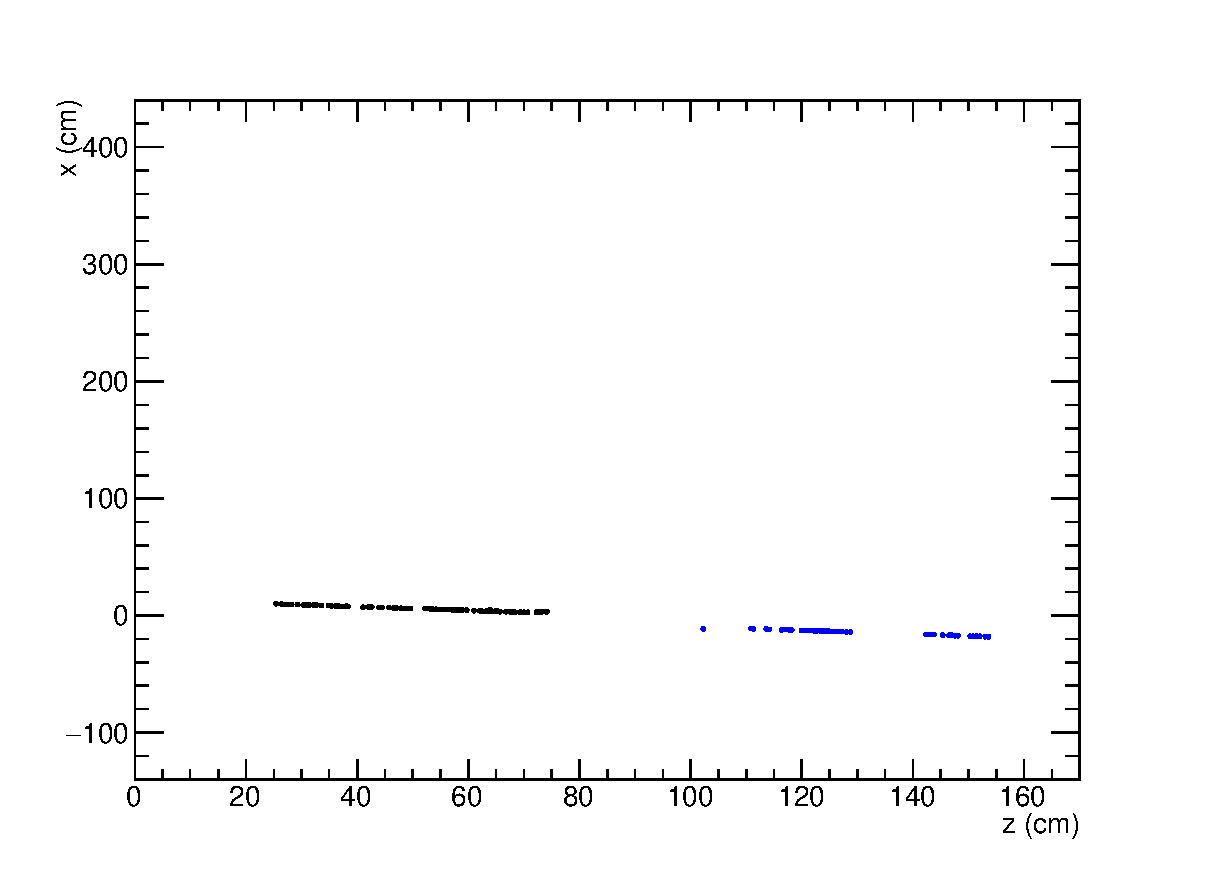
\includegraphics[width=\textwidth]{t0correction_before.eps}
    \caption{Correcting for $T_0^{\mathrm{counter}}$.}
    \label{fig:TPCCounterT0CorrectionCounter}
  \end{subfigure}
  \hfill
  \begin{subfigure}[t]{0.48\linewidth}
    \centering
    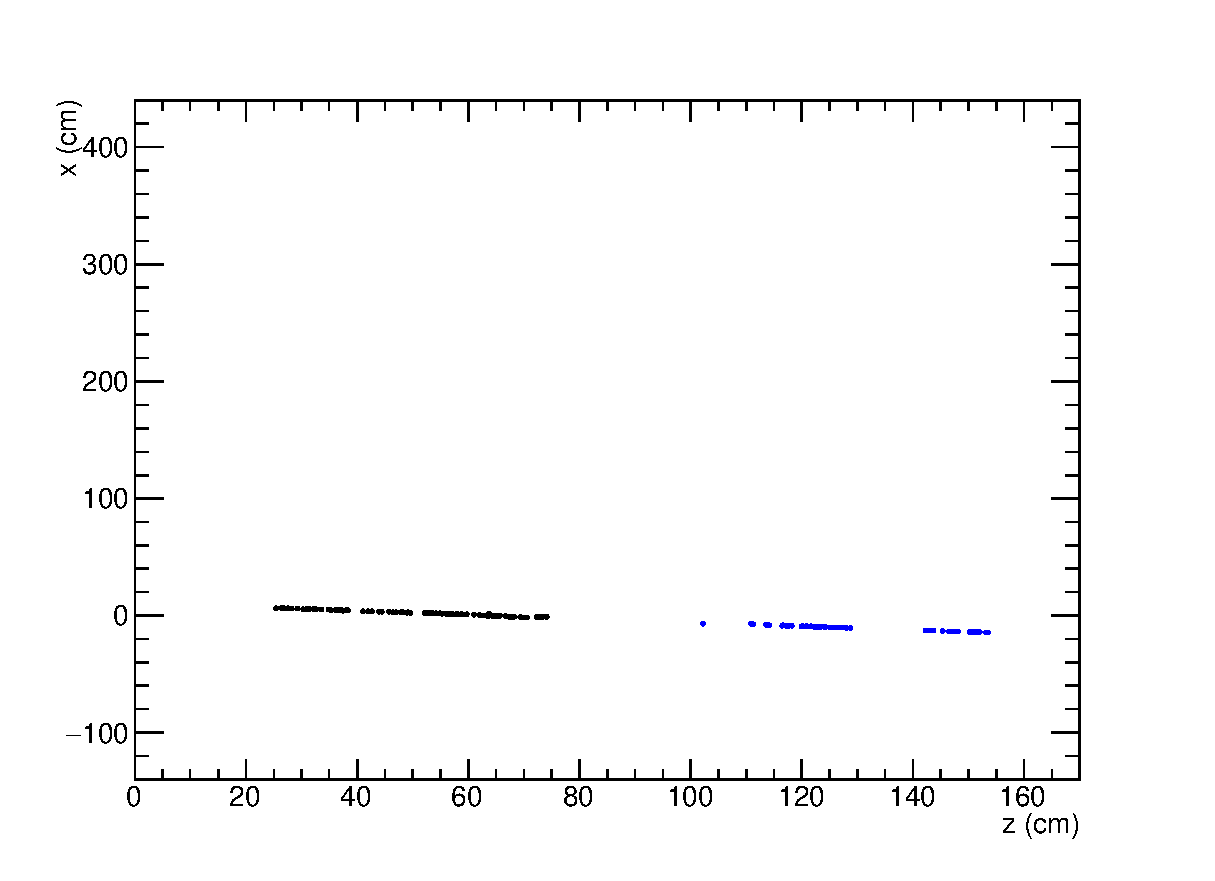
\includegraphics[width=\textwidth]{t0correction_after.eps}
    \caption{Correcting for $T_0^{\mathrm{TPC}}$.}
    \label{fig:TPCCounterT0CorrectionTPC}
  \end{subfigure}
  \caption[Correcting for T0 using $T_0^{\mathrm{counter}}$ and $T_0^{\mathrm{TPC}}$.]{Correcting for T0 using $T_0^{\mathrm{counter}}$ (Figure \ref{fig:TPCCounterT0CorrectionCounter}) and $T_0^{\mathrm{TPC}}$ (Figure \ref{fig:TPCCounterT0CorrectionTPC}).  The difference is subtle but obvious; the method for determining T0 directly from the TPC data can be validated by eye.  The minimisation of the metrics to determine $T_0^{\mathrm{TPC}}$ in this case are demonstrated in Figs. \ref{fig:APACrossingAlignmentLeastSqMin} and \ref{fig:APACrossingAlignmentSeparationMin}.}
  \label{fig:TPCCounterT0Correction}
\end{figure}

Attempts to understand the misalignment of the tracks across the APAs are presented in the remainder of this section.
%% the inconsistency between $T_0^{\mathrm{counter}}$ and $T_0^{\mathrm{TPC}}$ are presented in the remainder of this section.

%%%%%%%%%%%%%%%%%%%%%%%%%%%%%%%%%%%%%%%%%%%%%%%%%%%%%%%%%%%%%%%%%%%%%%%%%%%%%%%%%%%%%%%
\subsubsection{Understanding the Misalignment of APA Crossing Tracks}\label{sec:APACrossingMisalignment}

The underlying issue described above is essentially a misalignment of the same particle track between the two drift regions (see Figure \ref{fig:TrackMisalignment}).  This obviously is not physical and stems from an issue with the detector or data readout.  The most obvious cause is a miscalibration of the DAQ timing systems for the separate detector components, as previous assumed; there are however other possible causes for this problem.  Most likely, the effect arises from a combination of these different factors.

\begin{figure}[h]
  \centering
  \includegraphics[width=6cm]{misalign_track_geo.eps}
  \caption[Demonstration of the effect observed in the 35~ton data concerning tracks crossing the APAs.]{(Possibly unnecessary, but helps to explain all the various factors which could explain the offset. Can remake if necessary.) Demonstration of the effect observed in the 35~ton data concerning tracks crossing the APAs.  Even after correcting for the T0 provided by the counters, there is still a misalignment of the track segments across the APA frames.}
  \label{fig:TrackMisalignment}
\end{figure}

\paragraph{Geometry}

Apart from timing, a misunderstanding a the geometry could explain this perceived misalignment.  The spacing between the collection planes is one such example, as demonstrated in Figure \ref{fig:TrackMisalignmentCollectionSpacingGeo}; the spacing necessary to explain this affect, determined by aligning the tracks using the methods discussed above over a range of collection plane spacing hypotheses, is demonstrated in Figure \ref{fig:TrackMisalignmentCollectionSpacingRes}.  As is evident from the figure, the collection planes must be repositioned in such a way that they would be reversed; the track alignment complications cannot be explained solely by this.

\begin{figure}
  \centering
  \begin{subfigure}[t]{0.48\linewidth}
    \centering
    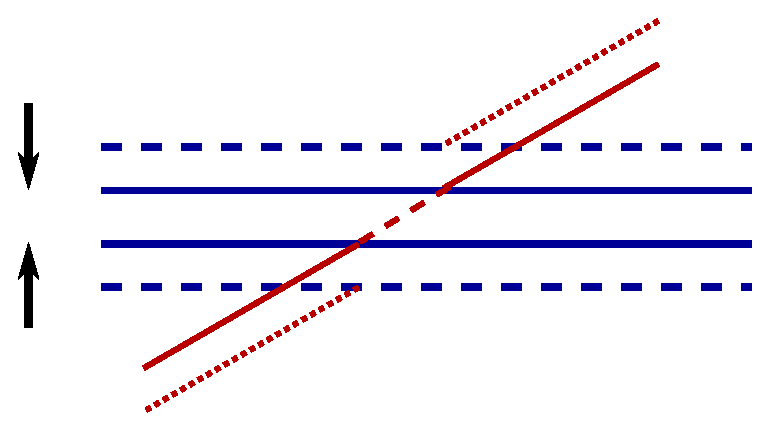
\includegraphics[width=\textwidth]{misalign_track_collection_geo.eps}
    \caption{Demonstration of how the track misalignment could be explained by an incorrect collection plane spacing.}
    \label{fig:TrackMisalignmentCollectionSpacingGeo}
  \end{subfigure}
  \hfill
  \begin{subfigure}[t]{0.48\linewidth}
    \centering
    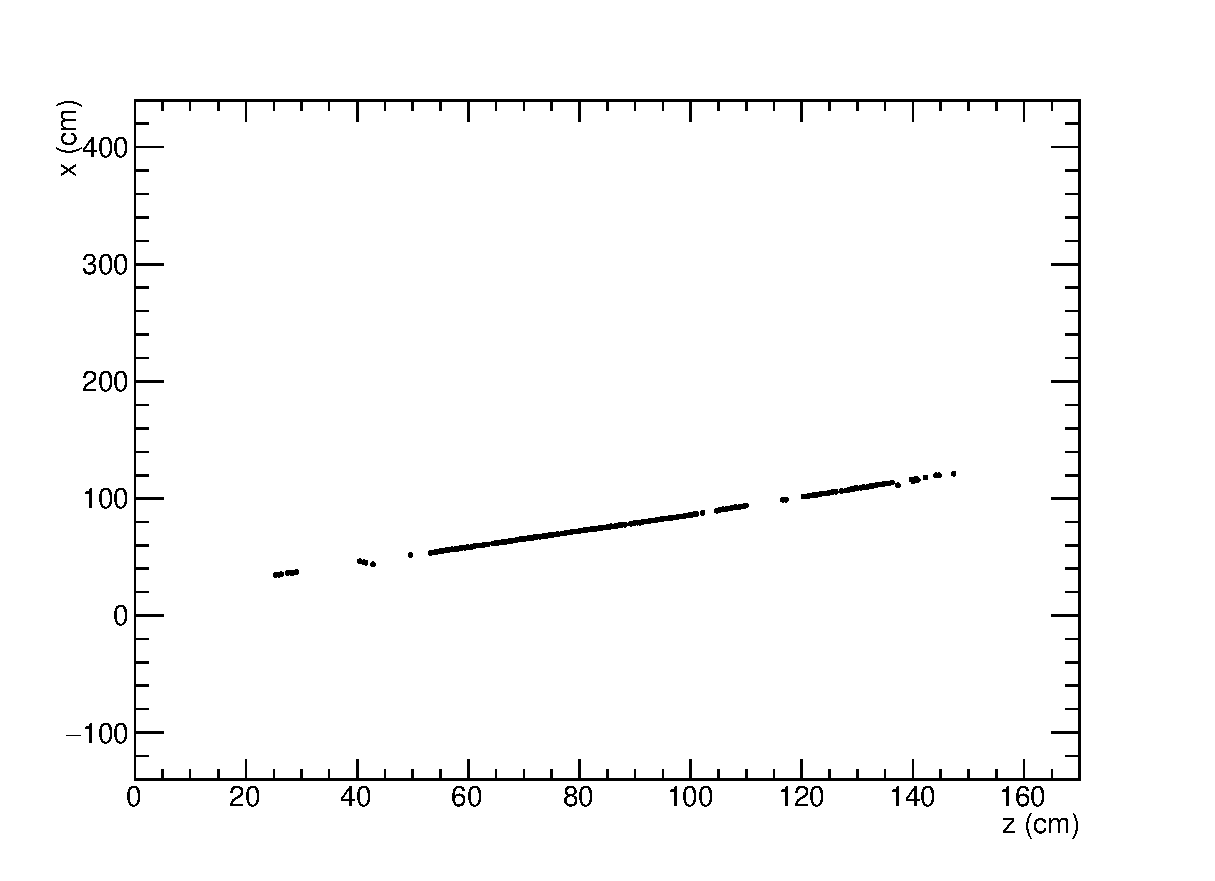
\includegraphics[width=\textwidth]{misalign_track_collection_res.eps}
    \caption{Corrected spacing between the collection planes after considering a range of values and aligning the track segments.  The red line shows the spacing used in the geometry.}
    \label{fig:TrackMisalignmentCollectionSpacingRes}
  \end{subfigure}
  \caption[Attemping to correct the track segment misalignment by assuming a misunderstanding of the spacing between the collection planes.]{Attemping to correct the track segment misalignment by assuming a misunderstanding of the spacing between the collection planes.  It appears the resulting spacing necessary to correct for this issue would involve physically reversing the order of the planes.}
  \label{fig:TrackMisalignmentCollectionSpacing}
\end{figure}

A further problem is related to the wire positioning on the APAs in the $z$-direction; it is understood there may be a discrepency between the two sides of the APA resulting in hits from the long and short drift regions at the same $z$-position reconstructed with a systematic offset.  Figure \ref{fig:TrackMisalignmentZPositionGeo} shows how this could be utilised to explain the apparent track misalignment with Figure \ref{fig:TrackMisalignmentZPositionRes} showing the distribution of corrected $z$ positions necessary to resolve the issue.  Offsets of $\sim30$~cm, as suggested by these results, are impossible, indicating again the track alignment problem cannot be resolved in this way.

\begin{figure}
  \centering
  \begin{subfigure}[t]{0.48\linewidth}
    \centering
    \includegraphics[width=\textwidth]{misalign_track_wire_geo.eps}
    \caption{Demonstration of how the track misalignment could be explained by an offset in the wire $z$-position on either side of the APA.}
    \label{fig:TrackMisalignmentZPositionGeo}
  \end{subfigure}
  \hfill
  \begin{subfigure}[t]{0.48\linewidth}
    \centering
    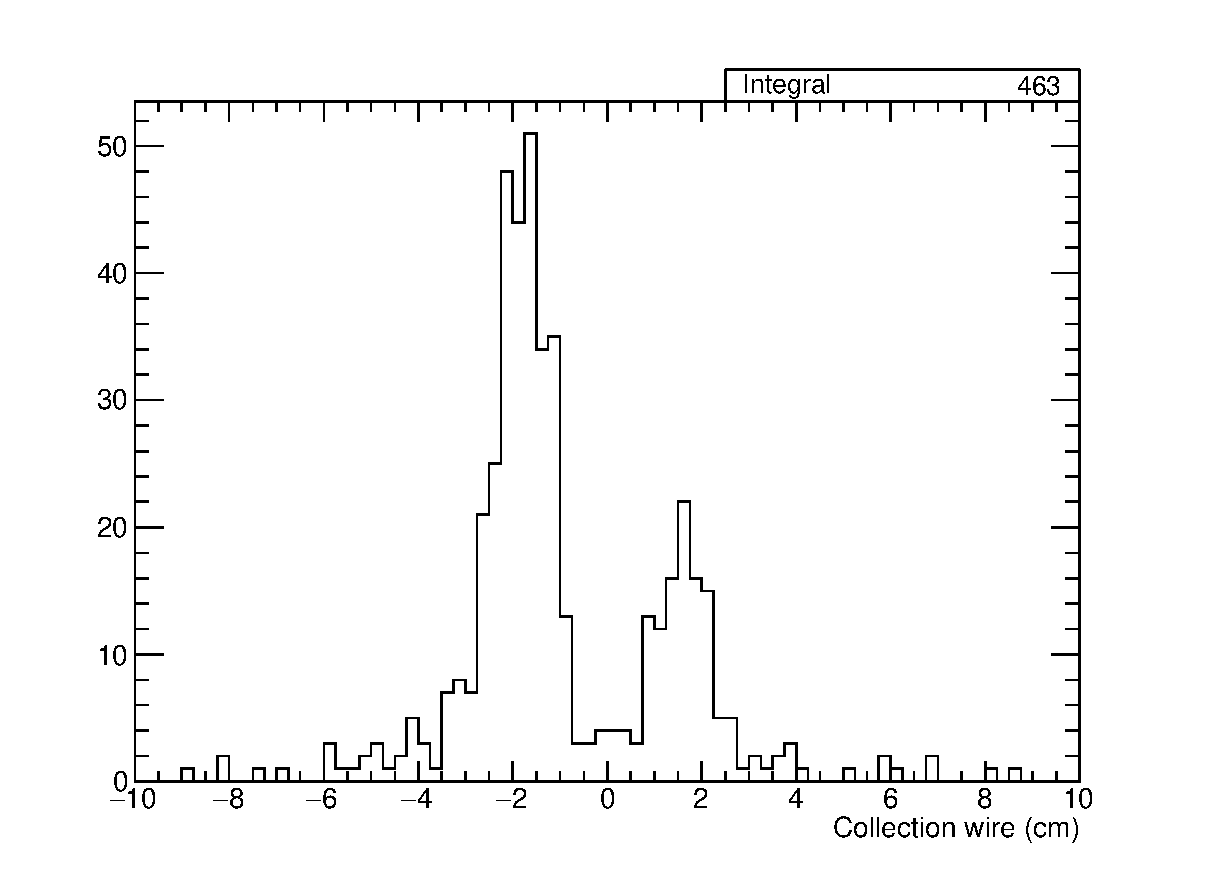
\includegraphics[width=\textwidth]{misalign_track_wire_res.eps}
    \caption{Corrected $z$-positions of the APA wires after considering a range of values and aligning the track segments.}
    \label{fig:TrackMisalignmentZPositionRes}
  \end{subfigure}
  \caption[Attempting to correct the track segment misalignment by assuming a misunderstanding of the positioning of the collection wires inside the detector.]{Attempting to correct the track segment misalignment by assuming a misunderstanding of the positioning of the collection wires inside the detector.  The wire offset would have to be around a foot to fix this issue.}
  \label{fig:TrackMisalignmentZPosition}
\end{figure}

\paragraph{Drift velocity}

The drift velocity affects the angle of the tracks in wire/time space; a high velocity would result in a refraction-like effect towards the APA planes.  As demonstrated in Figure \ref{fig:TrackMisalignmentDriftVelocityGeo}, this could explain the track segment misalignment if the effect was large enough.  Figure \ref{fig:TrackMisalignmentDriftVelocityRes} shows the necessary drift velocity required to account for the disparity observed in data; compared to a nominal value of $109$~cm/ms, the scale of the change required to explain the oddity is unreasonably large.

\begin{figure}
  \centering
  \begin{subfigure}[t]{0.48\linewidth}
    \centering
    \includegraphics[width=\textwidth]{misalign_track_drift_geo.eps}
    \caption{Demonstration of how the track misalignment could be explained by an incorrect drift velocity.}
    \label{fig:TrackMisalignmentDriftVelocityGeo}
  \end{subfigure}
  \hfill
  \begin{subfigure}[t]{0.48\linewidth}
    \centering
    \includegraphics[width=\textwidth]{misalign_track_drift_res.eps}
    \caption{Corrected drift velocity required to align the track across the APAs.}
    \label{fig:TrackMisalignmentDriftVelocityRes}
  \end{subfigure}
  \caption[Attempting to correct the track segment misalignment by assuming an incorrect drift velocity.]{Attempting to correct the track segment misalignment by assuming an incorrect drift velocity.  In order to account for the effect noted in the data the drift velocity would have to around five times larger than that initially calculated from models.}
  \label{fig:TrackMisalignmentDriftVelocity}
\end{figure}

This can be tested by measuring the drift velocity directly from the data.  Taking tracks which pass through opposite counter pairs and comparing this drift distance with drift time is a trivial exercise, demonstrated in Figure. \ref{fig:DriftVelocity}.  The measured value of $110$~cm/ms agrees exceptionally well with the aformentioned value, determined theoretically, of $109$~cm/ms.  It may therefore be assumed the drift velocity is as expected and does not contribute at all to the track alignment anomoly.

\begin{figure}
  \centering
  \begin{subfigure}[t]{0.48\linewidth}
    \centering
    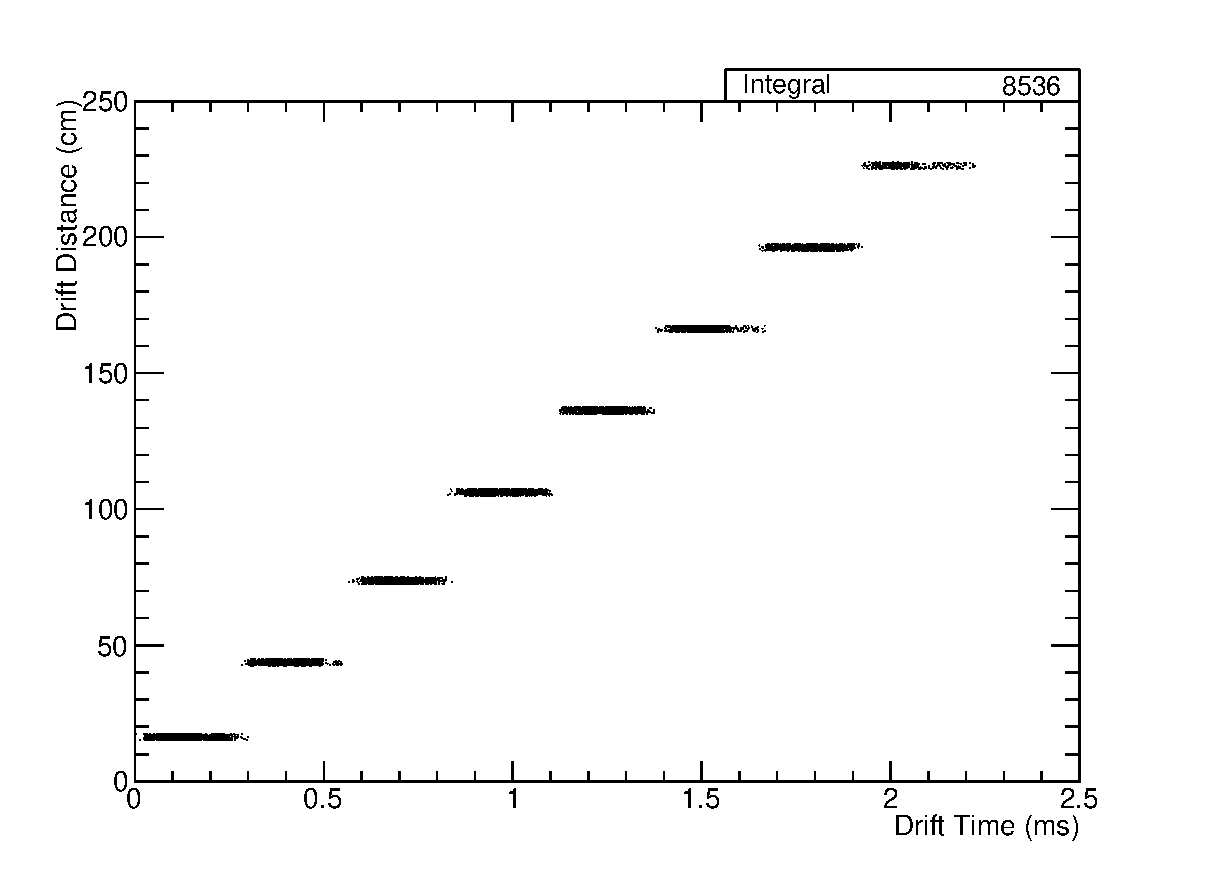
\includegraphics[width=\textwidth]{DistanceDriftTime.eps}
    \caption{Distribution of hit drift times for eight sets of counter pairs, assuming all tracks pass through the centres of the counters.}
    \label{fig:DistanceDriftTime}
  \end{subfigure}
  \hfill
  \begin{subfigure}[t]{0.48\linewidth}
    \centering
    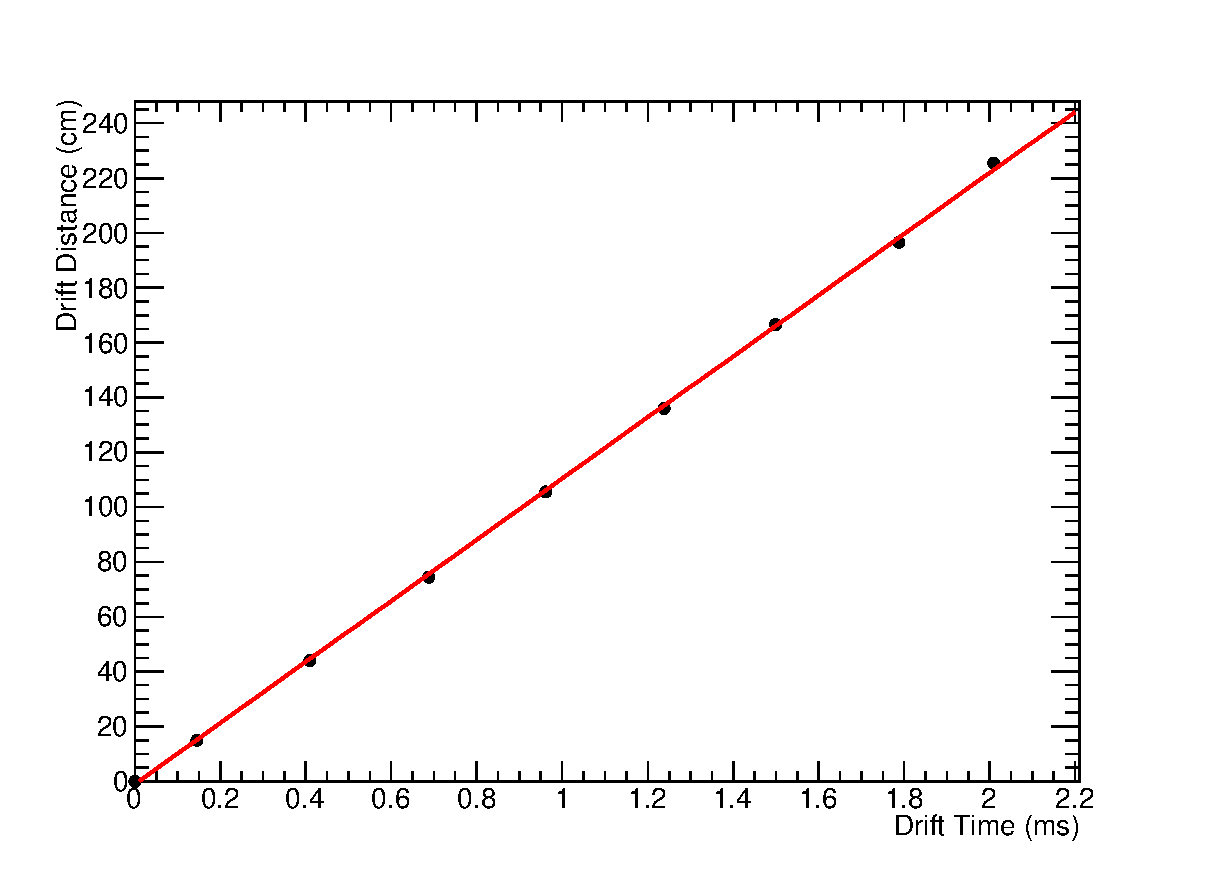
\includegraphics[width=\textwidth]{DriftVelocity.eps}
    \caption{The eight points found from taking the Gaussian mean of the time distributions for each rough drift distance.}
    \label{fig:DriftVelocityGraph}
  \end{subfigure}
  \caption[Measuring the drift velocity of the ionisation electrons by taking tracks passing through opposite counter pairs and comparing the corresponding drift distance to the drift time.]{Measuring the drift velocity of the ionisation electrons by taking tracks passing through opposite counter pairs and comparing the corresponding drift distance to the drift time.  Assuming all tracks pass through the geometric centres of the counters, a poor assumption, a distribution of hit time for this drift distance can be found; this is shown in \ref{fig:DistanceDriftTime}.  Taking each counter pair separately and fitting a Gaussian to the distribution of drift times nulifies the assumptions necessary due to a lack of exact knowledge, on a track by track basis, of the exact $x$-position.  This is shown in the graph in Figure \ref{fig:DriftVelocityGraph}.}
  \label{fig:DriftVelocity}
\end{figure}

\paragraph{Timing}

The timing offset calculated in Section. \ref{sec:APACrossingAlignment}, 32~$\mu$s, is so large it was assumed another explaination for the track segment misalignment was likely.  However, after reviewing all possibilities it appears there must be a significant timing offset present somewhere in the data.  Further evidence for this hypothesis is presented in Figure \ref{fig:HitTime} which displays the T0-corrected time distribution for all hits on the APA crossing track.  The minimum drift time these hits may have, since they pass directly through the planes, is the interaction time, T0.  As is evident from the distribution in Figure \ref{fig:HitTimeZoom}, this is around 56 ticks (28~$\mu$s) and is notably inconsistent with zero.  The curious spike at the interaction time motivates the work presented in Section \ref{sec:APACrossingCharge} and will be discussed there.

\begin{figure}
  \centering
  \begin{subfigure}[t]{0.48\linewidth}
    \centering
    \includegraphics[width=\textwidth]{HitTimes.eps}
    \caption{Over the full range of drift times.}
    \label{fig:HitTimeRange}
  \end{subfigure}
  \hfill
  \begin{subfigure}[t]{0.48\linewidth}
    \centering
    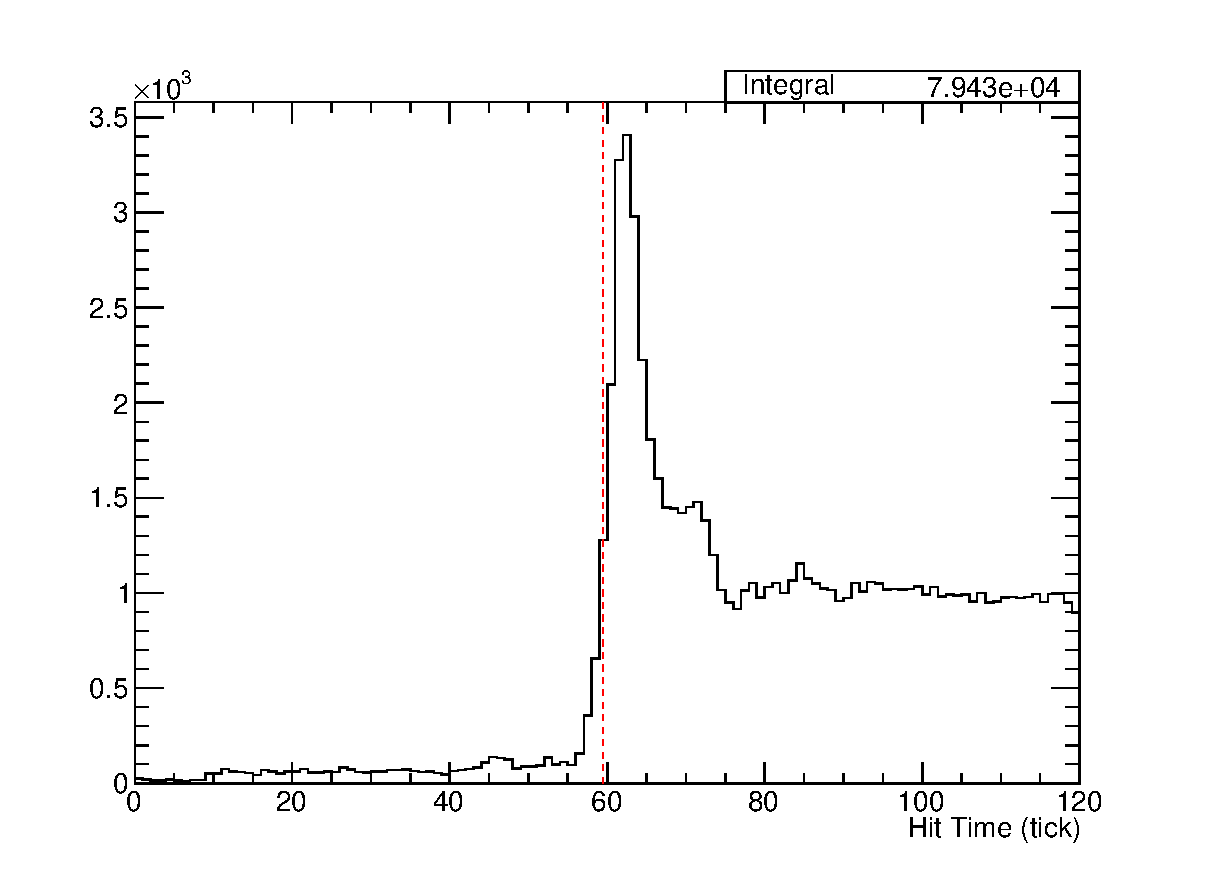
\includegraphics[width=\textwidth]{HitTimesZoom.eps}
    \caption{Zoomed in on the interaction time.}
    \label{fig:HitTimeZoom}
  \end{subfigure}
  \caption[The T0-corrected drift time for hits on APA crossing tracks.]{The T0-corrected drift time for hits on APA crossing tracks.  The lower leading edge of this distribution is an indication of the interaction time, T0.  The red line on Figure \ref{fig:HitTimeZoom} is drawn at 56 ticks (28~$\mu$s) and represents, by eye, the start of the distribution.}
  \label{fig:HitTime}
\end{figure}

This interesting result provoked further investigation into the notion of a timing offset between detector components, specifically the TPC and counter readout (RCEs and PTB respectively).  Confirmation of this miscalibration is displayed in Figure \ref{fig:TPCCounterOffset} which shows the difference between the timestamps recorded by each of the subcomponents upon recieving the trigger.

\begin{figure}[tb]
  \centering
  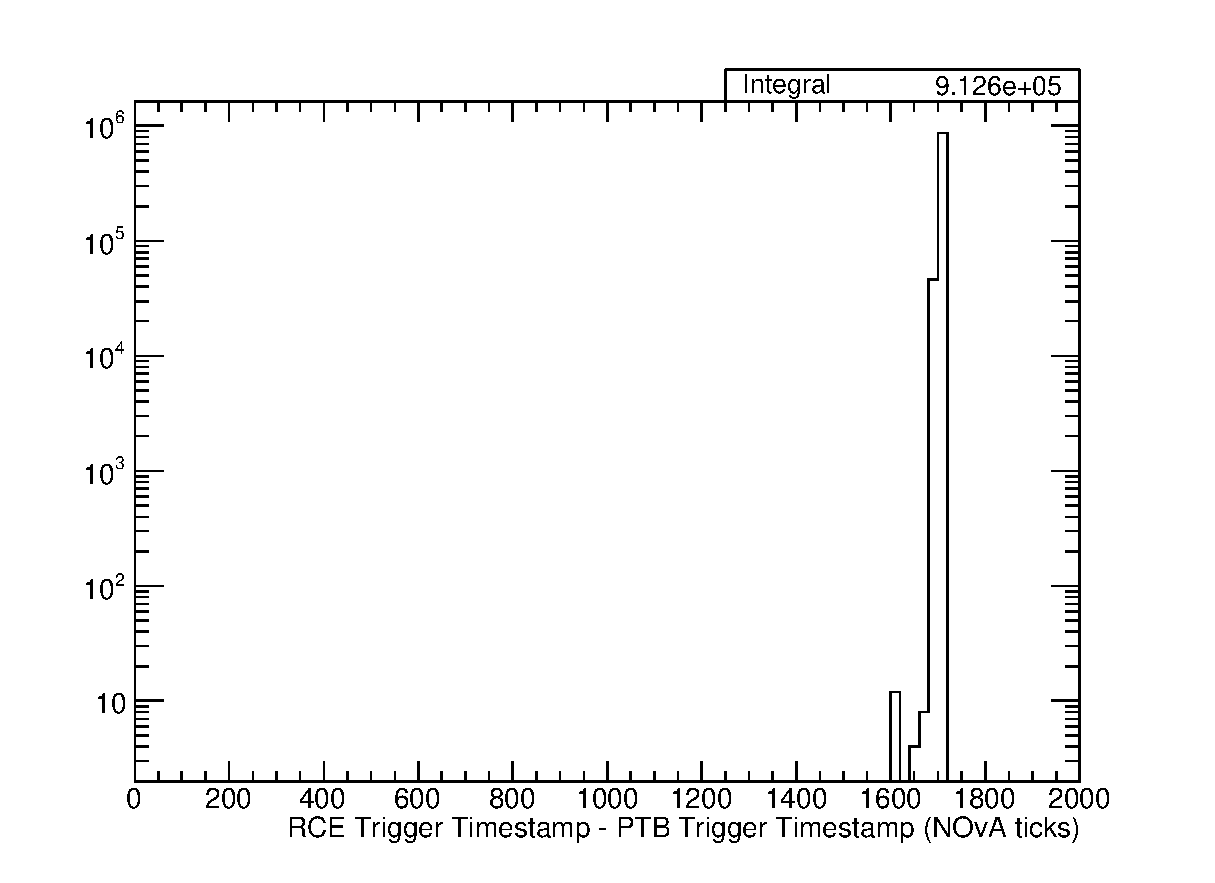
\includegraphics[width=12cm]{PTBRCEDiffTimestamps.eps}
  \caption[The difference between the timestamps recorded by the PTB and the RCEs upon recieving a trigger.]{The difference between the timestamps recorded by the PTB and the RCEs upon recieving a trigger.  The absolute timing for the DAQ system is given, along with most experiments at FNAL, by `NO$\nu$A time': a 64~MHz clock starting on 1st January, 2010 (with one NO$\nu$A tick therefore being 15.625~ns).  The distribution peaks sharply at 1705 NO$\nu$A ticks, or 26.6~$\mu$s.}
  \label{fig:TPCCounterOffset}
\end{figure}

Within the limitations of all methods discussed, there is agreement between the T0 offset in Figure \ref{fig:HitTimeZoom} and the timing miscalibration in Figure \ref{fig:TPCCounterOffset}.  This does not however account for the full track segment misalignment; this represents 64~ticks (32~$\mu$s) if accounted for using timing alone, as seen in Figure \ref{fig:TPCCounterT0Difference}.  As previously noted, the complete solution is likely a combination of different effects.  Given that drift velocity and $z$-position of wires effects are neglible, the remaining offset must be due to a slight discrepency between the actual spacing of the collection planes and what is being assumed.  With an actual T0 of 56 ticks, this collection plane spacing can be determined in the usual way by aligning tracks.  The results of this are demonstrated in Figure \ref{fig:RemainingCollectionSpacing}.

\begin{figure}[tb]
  \centering
  \caption{}
  \label{fig:RemainingCollectionSpacing}
\end{figure}

The misalignment of the tracks, as described in Section \ref{sec:APACrossingAlignment}, can be understood as a combination of a timing miscalibration between two detector components and a slight offset in the geometry, which is not unexpected.  This is the first time tracks crossing the readout planes have been used in a LArTPC experiment and have proven to be a valuable way of calibrating inter-detector components and finding other inconsistencies in the data.  Without studying this data set, the timing offset between the TPC and the external counters would not have been discovered and all analyses would naively use the incorrect T0.  In the next section, another source of information which can be gleaned from this dataset, this time more about understanding detector responses, will be discussed.

%%%%%%%%%%%%%%%%%%%%%%%%%%%%%%%%%%%%%%%%%%%%%%%%%%%%%%%%%%%%%%%%%%%%%%%%%%%%%%%%%%%%%%%
\subsection{Charge Deposited by APA Crossing Tracks}\label{sec:APACrossingCharge}

The intriguing distribution of the T0-corrected hit times observed in the data, shown in Figure \ref{fig:HitTimeRange}, hints at some aspect of the detector response that needs to be understood.  In the DUNE far detector, a large number of events will contain particles which pass through the APA frames so characterising resulting effects is critical.  The equivalent plot for simulated data, filtered by those triggered using external counters and processed in the same way, is shown in Figure \ref{fig:HitTimesMC}.  Comparing these distributions, there is a very obvious difference around the interaction time. It appears there is an effect present in the data, not currently being simulated, which manifests in around twice the amount of hits occurring at T0 on the collection planes for APA crossing tracks.  This is described in Section \ref{sec:InteractionTimeHits} and the phonomenon is visible on event displays presented in Section \ref{sec:HookEVDs}.

\begin{figure}
  \centering
  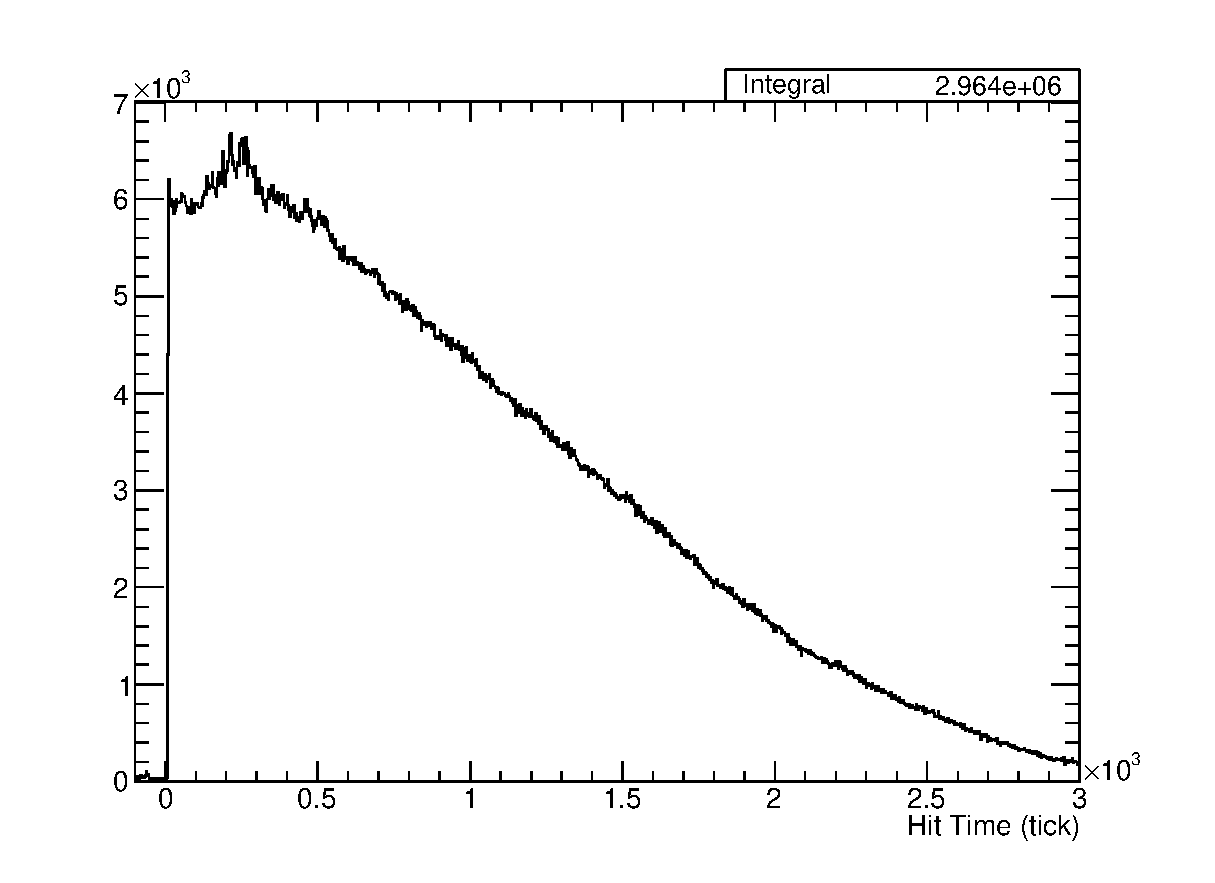
\includegraphics[width=12cm]{HitTimesMC.eps}
  \caption[The T0-corrected drift time for all hits on an APA crossing track in simulation.]{The T0-corrected drift time for all hits on an APA crossing track in simulation.  The equivalent plot for 35~ton data is shown in Figure \ref{fig:HitTimeRange}.}
  \label{fig:HitTimesMC}
\end{figure}

%%%%%%%%%%%%%%%%%%%%%%%%%%%%%%%%%%%%%%%%%%%%%%%%%%%%%%%%%%%%%%%%%%%%%%%%%%%%%%%%%%%%%%%
\subsubsection{Interaction Time Hits}\label{sec:InteractionTimeHits}

The excess of hits at the interaction time is due to the use of a grounded `mesh' at the centre of the APAs.  The purpose of such a design choice is to ensure a uniform electric field across the face of the APA; without it the field would be ill-defined given the presence of the grounded, rectangular APA frames with positively biased planes on either side.  It is plausible therefore to consider a `backward-facing' field being set up between the grounded mesh and the positively biased collection planes which would lead to hits drifting the `wrong' way when produced in this region; APA crossing tracks would hence leave twice as many hits on the collection plane as the other planes.  This is demonstrated schmatically in Figure \ref{fig:MeshHits}.

\begin{figure}[p]
  \centering
  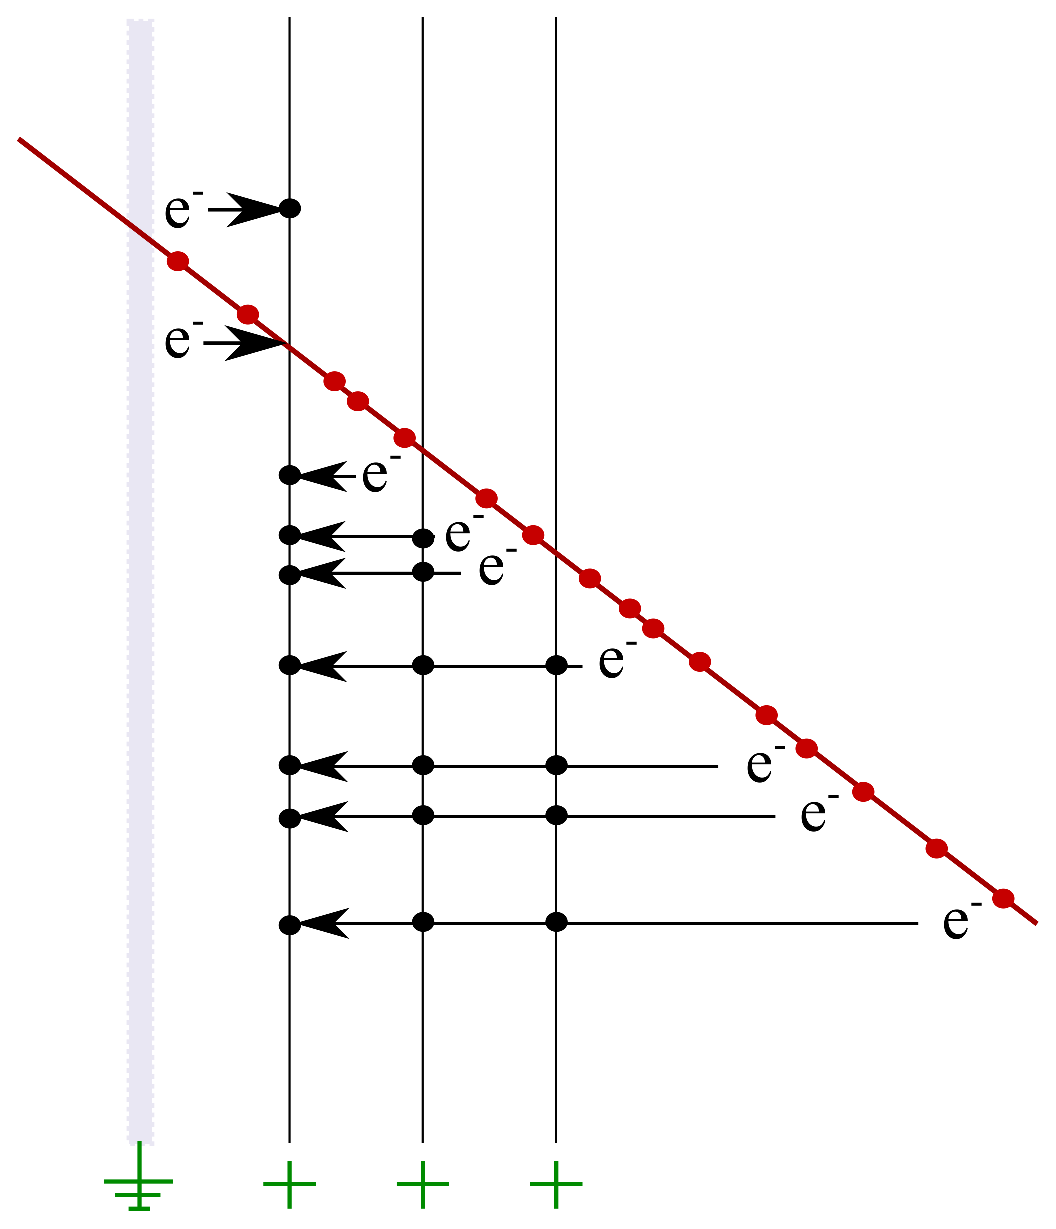
\includegraphics[width=12cm]{MeshHits.eps}
  \caption[Demonstration of the electron ionisation and hit collection for APA crossing tracks.]{Demonstration of the ionisation and hit collection for APA crossing tracks.  The red line represents a track passing through the anode planes, shown in black.  The grey region is the centre of the APA frame on which the grounded mesh is afixed.  The red dots correspond to the ionisation of electrons which then drift, depositing charge (black dots) on the readout wires.  The three planes shown are, from left to right, the collection plane and the two induction planes.  The biasing of each of the planes and mesh sets up field lines which all terminate on the collection wires, resulting in charge collected from before the track passes through and after.}
  \label{fig:MeshHits}
\end{figure}

A convenient way of confirming whether or not the mesh can explain this excess of hits at the interaction time is possible since one of the four APAs in the 35~ton was constructed without the mesh, precisely for this purpose.  Unfortunately, this was the APA which was more plagued by noise issues so very little good data is available from channels on this APAs.  It is however possible to make a crude comparison; this is shown in Figure \ref{fig:HitTimesAPAs}.  The appears to confirm the shark peak of hits occurring at the interaction time comes from the APAs which use a mesh.

\begin{figure}[htb]
  \centering
  \begin{subfigure}[t]{0.48\linewidth}
    \centering
    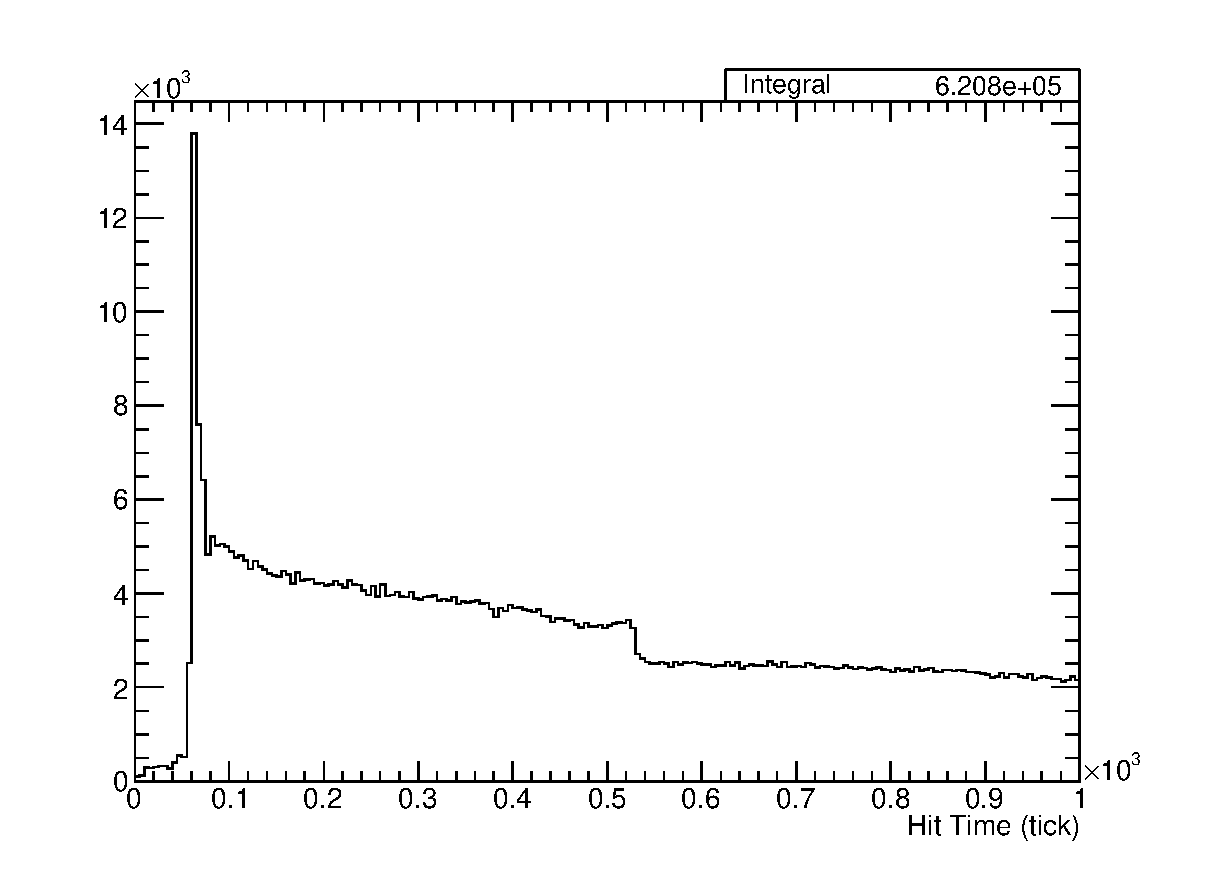
\includegraphics[width=\textwidth]{HitTimesAPA023.eps}
    \caption{Hit times for all hits on APAs 0, 2 and 3; these are the three APAs containing the grounded mesh at the centre.}
    \label{fig:HitTimesAPA023}
  \end{subfigure}
  \hfill
  \begin{subfigure}[t]{0.48\linewidth}
    \centering
    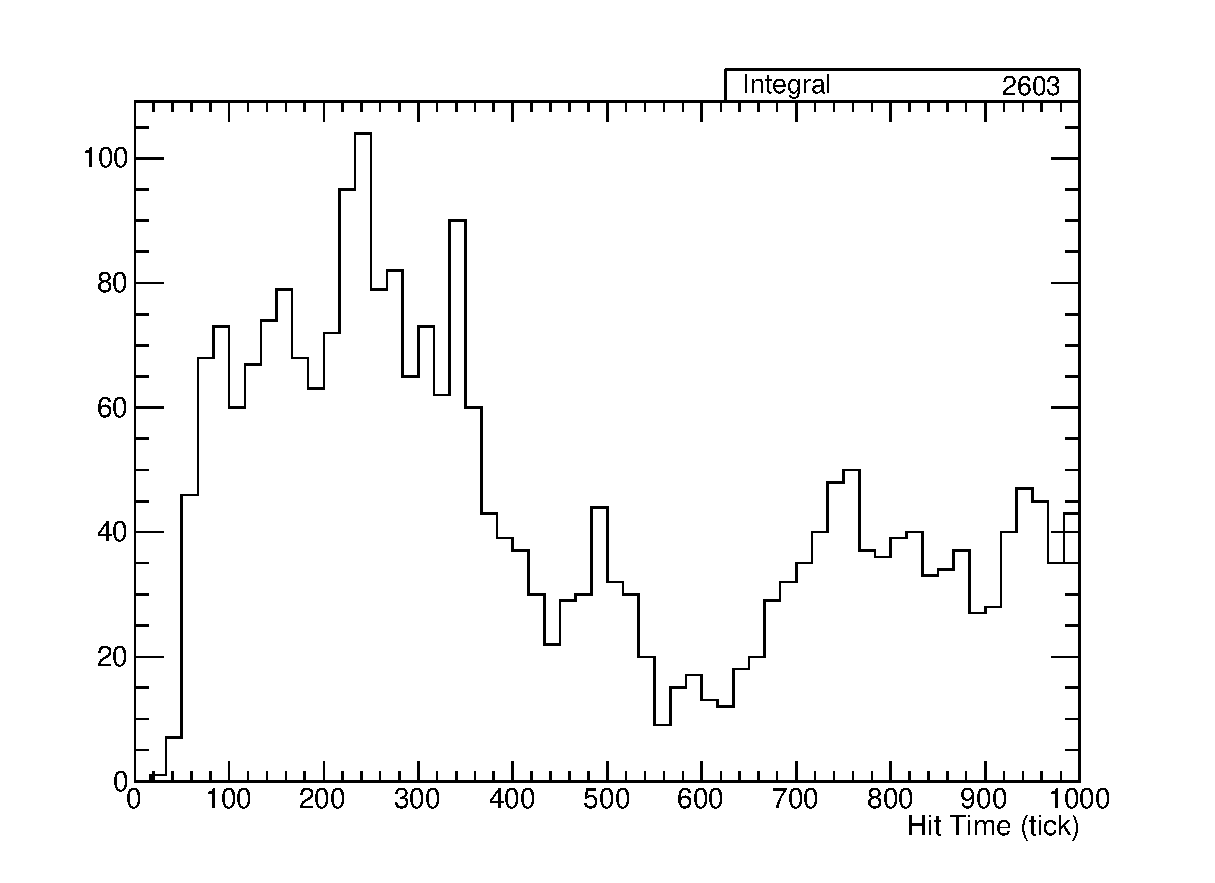
\includegraphics[width=\textwidth]{HitTimesAPA1.eps}
    \caption{Hit times for all hits on APA 1, the APA without a grounded mesh at its centre.}
    \label{fig:HitTimesAPA1}
  \end{subfigure}
  \caption[Comparison between the T0-corrected hit time distributions on APAs with and without the grounded mesh.]{Comparison between the T0-corrected hit time distributions on APAs with and without the grounded mesh.  Even given the very low stats in Figure \ref{fig:HitTimesAPA1}, there is a noticable difference in the distribution of hits around the interaction time.}
  \label{fig:HitTimesAPAs}
\end{figure}

Using the 35~ton dataset, it is also possible to confirm that the mesh is functioning as expected.  Without a mesh, one may expect a difference between the hits deposited on wires towards the centre of an APA face and wires at the edges, in front of the grounded frame.  The functionality of the grounded mesh ensures there is no difference between any wires on a given APA.  Figure \ref{fig:HitTimesFrame} comfirms this is the case.

\begin{figure}
  \centering
  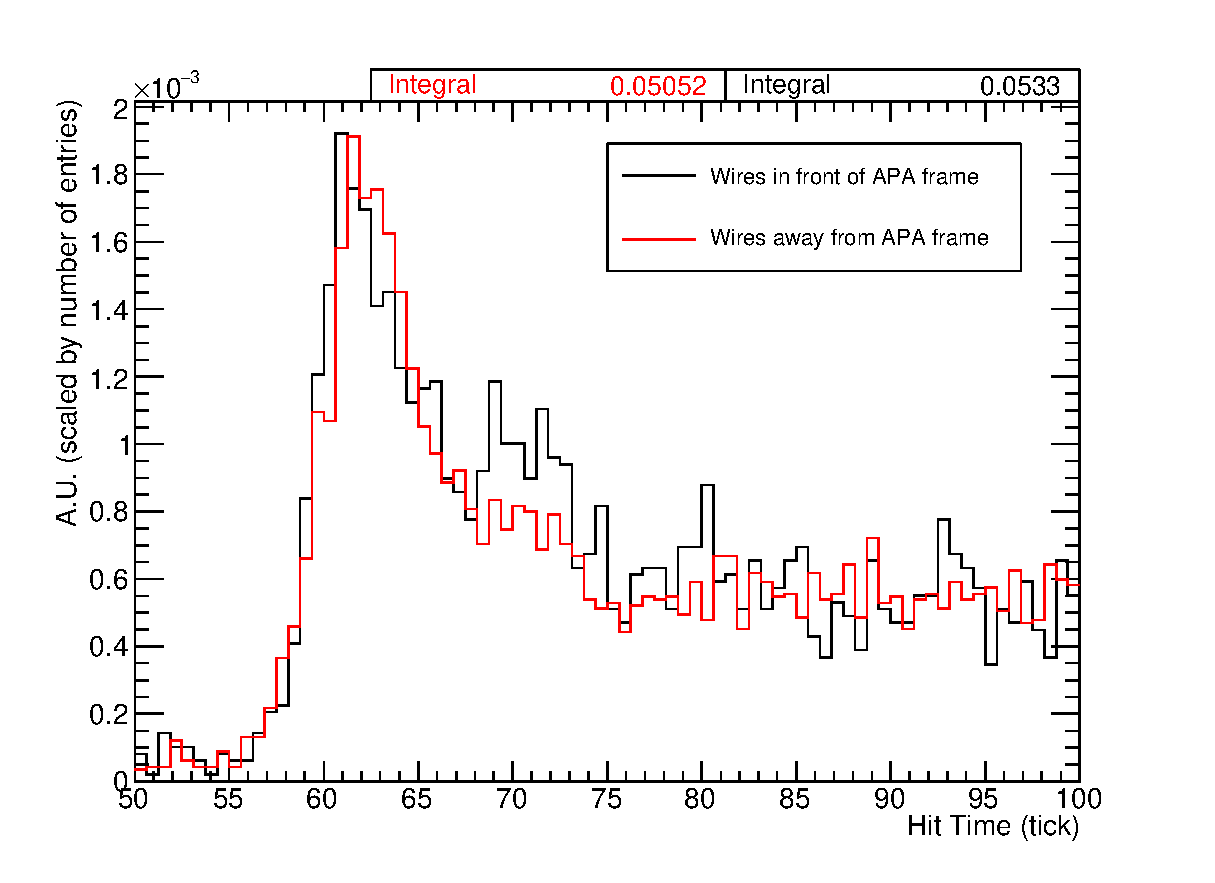
\includegraphics[width=10cm]{HitTimesFrame.eps}
  \caption[Comparison between the distribution of T0-corrected hit times for hits on wires in front of the APA frame and away from the APA frame to validate the functionality of the mesh.]{Comparison between the distribution of T0-corrected hit times for hits on wires in front of the APA frame and away from the APA frame to validate the functionality of the mesh.  Both distributions are normalised by the number of entries.  There is no evidence of any differences between the two distributions so this suggests the mesh is working as intended.}
  \label{fig:HitTimesFrame}
\end{figure}

A natural question to pose at this point is to ask if these `extra' hits deposited by APA crossing tracks as a result of this `backwards' field have similar properties to the `correct' hits.  The most important property to consider is the charge of the hits; Figure \ref{fig:HitCharges} shows the average charge per hit for hits occurring at the interaction time and all other hits.  It is clear from this there is nothing different about these additional hits and they can be treated in the same way.

\begin{figure}
  \centering
  \begin{subfigure}[t]{0.48\linewidth}
    \centering
    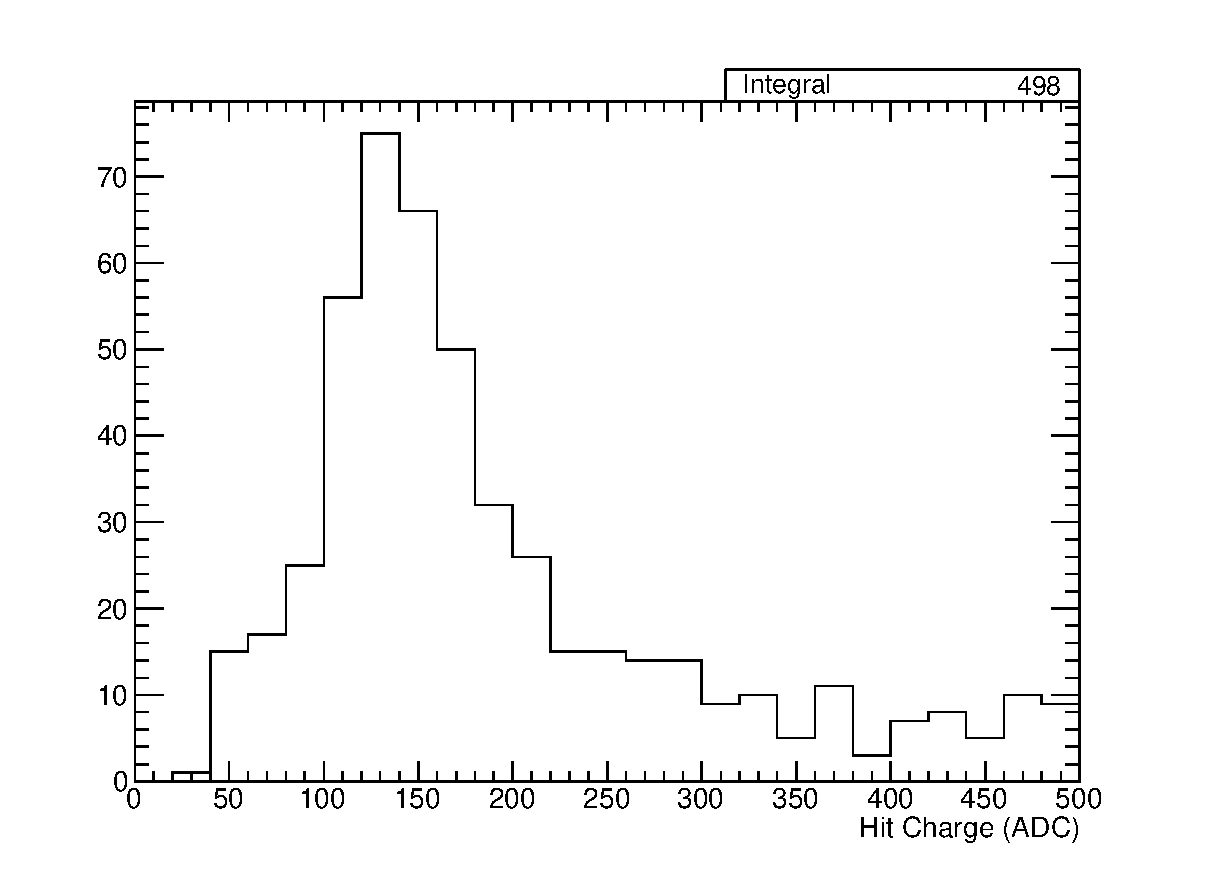
\includegraphics[width=\textwidth]{HitChargeInteraction.eps}
    \caption{Hits occurring around the interaction time; 50 < tick < 70.  A fitted Gaussian of the peak yields a mean of 149 and width of 49.}
    \label{fig:HitChargeInteraction}
  \end{subfigure}
  \hfill
  \begin{subfigure}[t]{0.48\linewidth}
    \centering
    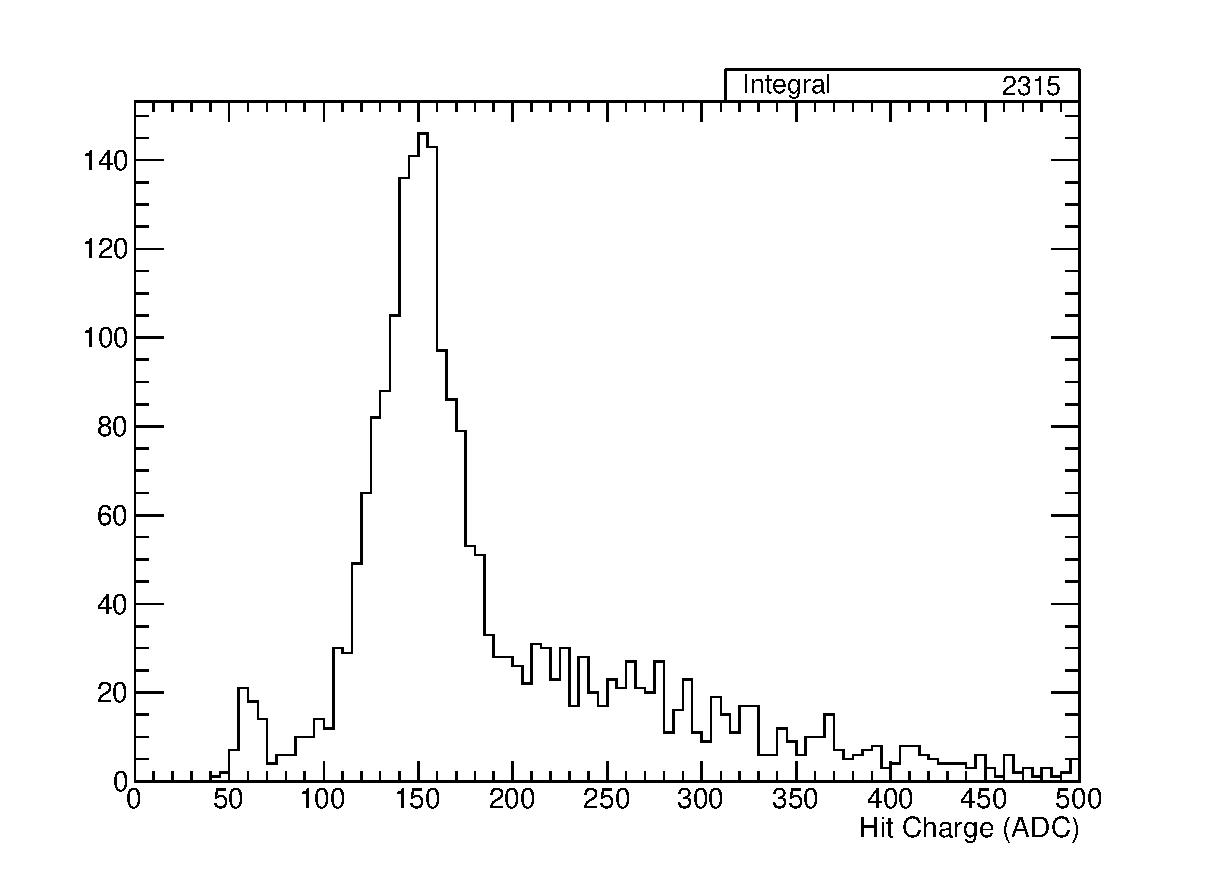
\includegraphics[width=\textwidth]{HitChargeNonInteraction.eps}
    \caption{Hits occurring away from the interaction time; tick < 50, tick > 70.  A fitted Gaussian of the peak yields a mean of 152 and a width of 28.}
    \label{fig:HitChargeNonInteraction}
  \end{subfigure}
  \caption[Average lifetime-corrected charge per hit for hits on an APA crossing track separated according to whether or not the hit was collected around the interaction time.]{Average lifetime-corrected charge per hit for hits on an APA crossing track separated according to whether or not the hit was collected around the interaction time.  There is no evidence to suggest the `extra' hits collected around the interaction time have significantly more or less average charge than `regular' hits.}
  \label{fig:HitCharges}
\end{figure}

As alluded to earlier, the DUNE simulation software is simplistic and does not simulate any ionisations within the region of the APA planes; in the case of APA crossing muons this results in no hits being created after the track passes through the first induction wires.  Evidently, this is an important region and must be understood and well simulated in order to test reconstruction and analyses.  When this is added to the software, the 35~ton data will be essential for validation purposes.

%%%%%%%%%%%%%%%%%%%%%%%%%%%%%%%%%%%%%%%%%%%%%%%%%%%%%%%%%%%%%%%%%%%%%%%%%%%%%%%%%%%%%%%
\subsubsection{Event Displays of APA Crossing Tracks}\label{sec:HookEVDs}

The effect investigated in Section \ref{sec:InteractionTimeHits} is directly observable in the raw data, as shown in Figure \ref{fig:HookEVDBig}.  The electrons ionised as the particle track passes between the collection plane and the mesh are observable as hits which appear to have drifted in the negative time direction.  The outcome is a little `hook' shape in the data.

%%%%%%%%%%%%%%%%%%%%%%%%%%%%%%%%%%%%%%%%%%%%%%%%%%%%%%%%%%%%%%%%%%%%%%%%%%%%%%%%%%%%%%%
\subsection{Comparison Between Drift Regions Using APA Crossing Tracks}\label{sec:APACrossingDriftComparison}

APA crossing tracks may be utilised to make unique, specific measurements of the detector made possible since they originate from the same particle.  For example, any drift velocity differences between the drift regions may be observed and the noise levels on the collection readouts on either side of the APA can be studied and compared.

The drift velocity is given by the angle of the track in wire/time space and any difference between this velocity in the two drift regions would be noticable in a refraction-like effect.  This is demonstrated in Figure \ref{fig:DriftVelocityDiffGeo}.  A measure of the angle between the track segments in the different regions would therefore be a measure of the change in drift velocity; this is shown in Figure \ref{fig:DriftVelocityDiffRes}.

\begin{figure}
  \centering
  \begin{subfigure}[t]{0.48\linewidth}
    \centering
    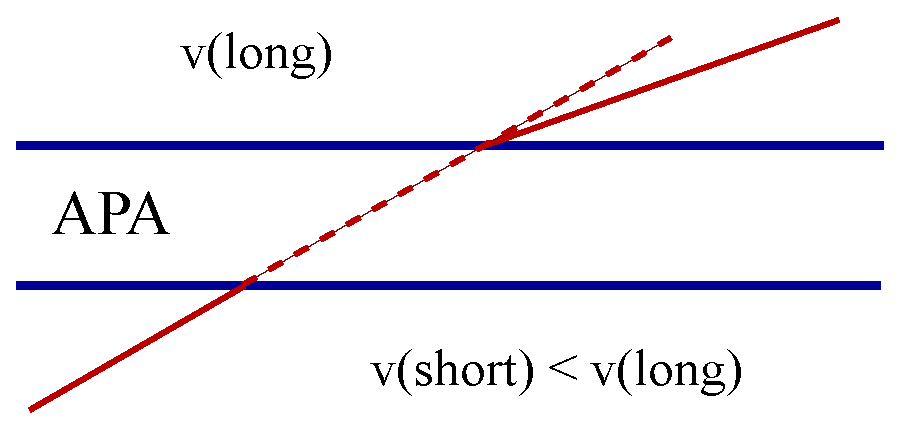
\includegraphics[width=\textwidth]{DriftVelocityDiffGeo.eps}
    \caption{}
    \label{fig:DriftVelocityDiffGeo}
  \end{subfigure}
  \hfill
  \begin{subfigure}[t]{0.48\linewidth}
    \centering
    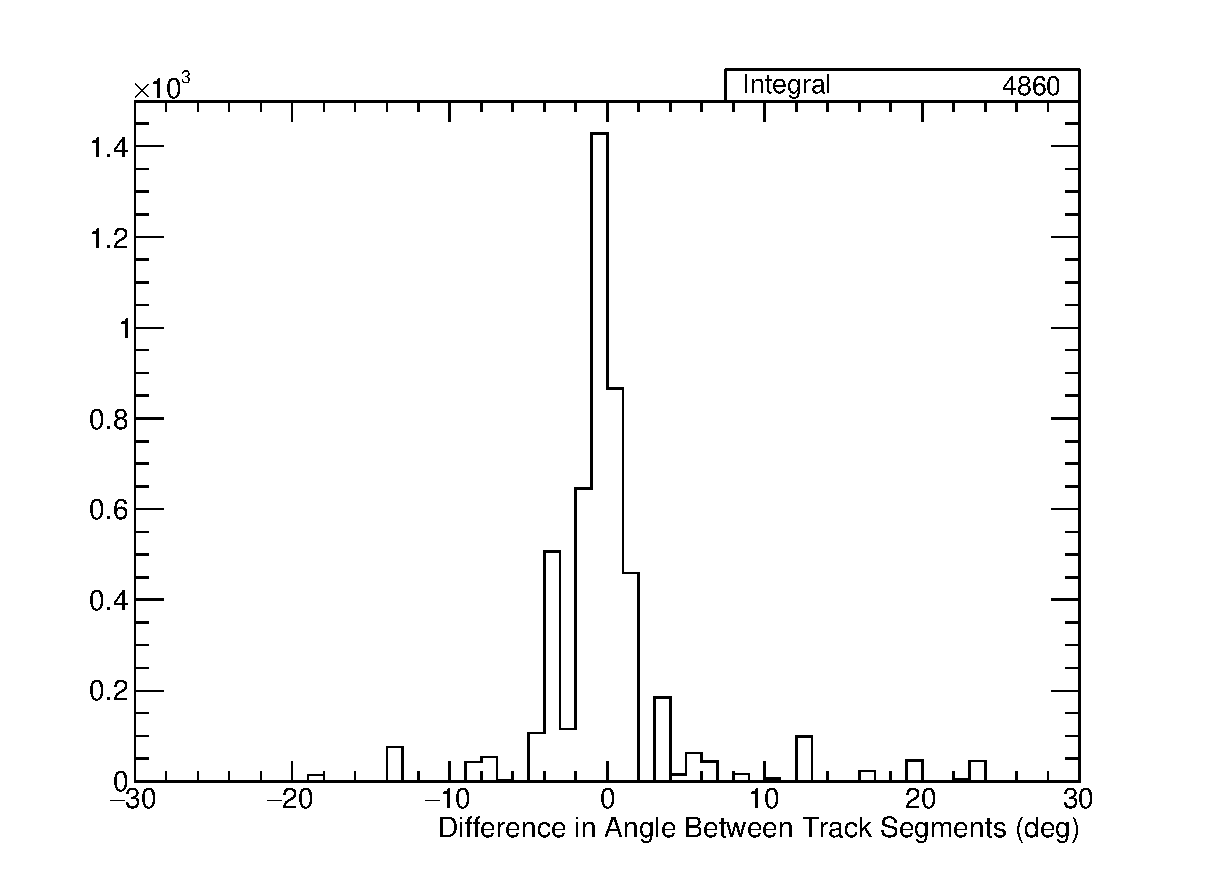
\includegraphics[width=\textwidth]{DriftVelocityDiffRes.eps}
    \caption{}
    \label{fig:DriftVelocityDiffRes}
  \end{subfigure}
  \caption[]{}
  \label{fig:DriftVelocityDiff}
\end{figure}

The relative noise on the two collection planes can be evaluated by considering the number of hits present in the counter shadow, in each drift region, which were not reconstructed as part of the track associated with the triggering particle.  The difference between each collection plane for a given event should peak at zero if similar levels of noise were observed in each drift region; this is confirmed in Figure \ref{fig:CollectionPlaneNoise}.

%% \begin{figure}
%%   \centering
%%   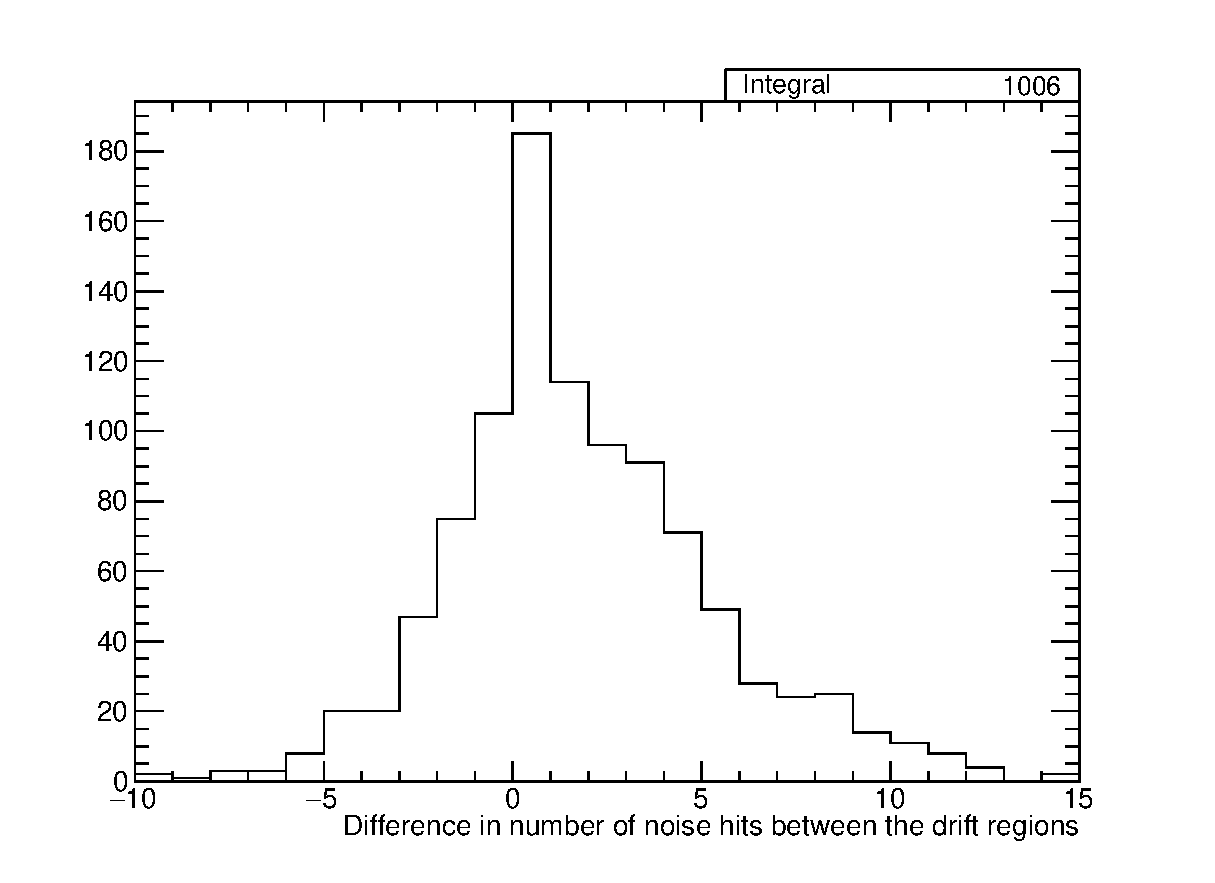
\includegraphics[width=10cm]{CollectionPlaneNoise.eps}
%%   \caption{}
%%   \label{fig:CollectionPlaneNoise}
%% \end{figure}

%%%%%%%%%%%%%%%%%%%%%%%%%%%%%%%%%%%%%%%%%%%%%%%%%%%%%%%%%%%%%%%%%%%%%%%%%%%%%%%%%%%%%%%
\section{APA Gap-Crossing Muons}\label{sec:APAGapCrossing}

One of the primary motivations for the design of the 35~ton TPC was to test the modular design, where a single drift region is read out by multiple anode assemblies.  Particles passing through the detector will inevitably leave deposits in multiple TPCs and will pass uninstrumented regions of the detector, such as gaps in between neighbouring APAs.  It is essential the implications of this design choice are understood before constructing the far detector modules, each of which will contain 150 APAs.

The 35~ton dataset consisting of muons which pass across the face of APAs and therefore deposit charge in consequetive TPCs is discussed in this present section.  An analysis of these tracks to calculate the size of the gaps is presented in Section \ref{sec:APAGapOffsets} and a study of the charge deposited by such tracks is the subject of Section \ref{sec:APAGapCharge}.

%%%%%%%%%%%%%%%%%%%%%%%%%%%%%%%%%%%%%%%%%%%%%%%%%%%%%%%%%%%%%%%%%%%%%%%%%%%%%%%%%%%%%%%
\subsection{APA-Gap Offset Determination}\label{sec:APAGapOffsets}

%%%%%%%%%%%%%%%%%%%%%%%%%%%%%%%%%%%%%%%%%%%%%%%%%%%%%%%%%%%%%%%%%%%%%%%%%%%%%%%%%%%%%%%
\subsection{Charge Deposited by APA-Gap Crossing Muons}\label{sec:APAGapCharge}

%%%%%%%%%%%%%%%%%%%%%%%%%%%%%%%%%%%%%%%%%%%%%%%%%%%%%%%%%%%%%%%%%%%%%%%%%%%%%%%%%%%%%%%
\section{Shower Reconstruction in 35~ton Data}\label{sec:ShowerData}
